\chapter{Velocity-space Tomography}\label{chap:velocity-space_tomography}

The previous chapter discussed the theoretical underpinnings of diagnostic weight functions. In this and the next chapter, we discuss their main application: the inference of the fast-ion distribution function from experimental measurements. As an appetizer for the main course of this thesis, Orbit Tomography, we will first discuss its precursor Velocity-space Tomography.

\section{Mathematical Formulation}
Velocity-space tomography, as the name suggests, uses velocity-space weight functions to infer a local approximation of the fast-ion distribution function---the distribution is local and approximate because, as we showed in the previous chapter, the weight functions are local and approximate.
Equation \ref{eq:vs_WF} can be discretized to form
\begin{equation} \label{eq:wf_discrete_single}
    s = \mathbf{w}^T \cdot \mathbf{f}\,,
\end{equation}
where $s$ is a scalar representing the measured signal, and the vectorized form of the velocity-space weight function and the local fast-ion distribution is given by $\mathbf{w}$ and $\mathbf{f}$ respectively. Equation \ref{eq:wf_discrete_single} alone is insufficient to infer a meaningful distribution function.
Since one pixel distributions are of limited use, multiple measurements and their corresponding weight functions are combined to create a system of linear equations:
\begin{equation}\label{eq:wf_discrete}
    \mathbf{s} = \mathbf{W}\cdot\mathbf{f}\,,
\end{equation}
where $\mathbf{s}$ is a column vector of the measurements and $\mathbf{W}$ is a weight matrix where each $i^{th}$ row contains the weight function, $\mathbf{w}_i^T$, for the $i^{th}$ measurement, $s_i$. 
The number of elements of $\mathbf{f}$, which are colloquially called ``pixels'', are chosen to to be less than the number of measurements available in order to create an over-determined system of equations. 
Ideally, the value of $\mathbf{f}$ is found by solving the over-determined system of equations; however, this is not the case in practice. Measurement noise and model inaccuracies prevent a direct application of linear algebra, requiring different methods to invert Equation \ref{eq:wf_discrete}. It is fortunate then that the tomographic techniques that have been used in plasma physics research in the past, provide a rich library of inversion methods to try.\cite{nagayama1981soft,koslover1986measurement,mcwilliams1987laboratory,reinhold1990excitation,Anton1996,zimmerman2005two,svensson2008current,odstrcil2012modern}

Forms of tomographic reconstructions has been used in plasma physics research for a number of decades; however,
despite the long history, a single best method has not emerged. This is because every tomography application is different. An inversion method well suited for one application may not be suitable for a different application. This is particularly true for Velocity-space Tomography since, unlike other types of tomography that use many measurements that are averaged over a line-of-sight, we use relatively few measurements that are averaged over a 2D area or, in the case of Orbit Tomography, a 3D volume. This precludes certain types of inversion methods, such as Radon transforms. It also makes tomography much more difficult since the many line-of-sight measurements of traditional tomography provide excellent discriminating information, which shrinks the possible set solutions significantly; the same cannot be said of the 2D/3D ``lines-of-sight'' of fast-ion tomography.

In order to determine their suitability for Velocity-space Tomography, in the following sections we will explore five different inversion methods that have been used in other applications and benchmark them against known theoretical distribution functions. We will then use the different methods to study the redistribution of fast-ions by a sawtooth crash. 

\section{Inversion methods}\label{sec:methods}
Measurement noise, error incurred by discretizing velocity-space, and the inherent flaws of velocity-space weight functions discussed in the previous chapter prevent an exact solution to Equation \ref{eq:wf_discrete}. We can instead use a probabilistic approach. Let's assume that the measured data, $\mathbf{s}$, is distributed according to a multivariate normal distribution,
\begin{equation}\label{eq:likelihood}
    \rm{prob}(\mathbf{s}|\mathbf{f},\mathbf{\Sigma}) \propto \exp{\left(-\frac{1}{2} (\mathbf{W}\cdot\mathbf{f} - \mathbf{s})^T \cdot \mathbf{\Sigma}^{-1} \cdot (\mathbf{W}\cdot\mathbf{f} - \mathbf{s})\right)}\,,
\end{equation}
where $\mathbf{\Sigma}$ is a diagonal matrix containing the variance/noise of the measured data. This probability is also known as the likelihood. We would like to find the value of $\mathbf{f}$ that maximizes the probability of observing the data. This can be reformulated as a minimization of the log-probability, which is equivalent to the classic least-squares minimization:
\begin{equation}\label{eq:least_squares}
    \mathrm{minimize} \left \lbrace \frac{1}{2}\left|\left| \mathbf{\overline{W}}\cdot\mathbf{f} - \mathbf{\overline{s}}\right|\right|^2 \right \rbrace 
\end{equation}
where the barred variables are normalized quantities: $\mathbf{\overline{W}} = \sqrt{\mathbf{\Sigma}^{-1}}\cdot\mathbf{W}$ and $\mathbf{\overline{s}}=\sqrt{\mathbf{\Sigma}^{-1}}\cdot\mathbf{s}$.
The minimum, $\mathbf{\hat{f}}$, of the above equation can be found analytically and is given by
\begin{equation}\label{eq:least_squares_solution}
    \mathbf{\hat{f}} = \left(\mathbf{\overline{W}}^T\cdot\mathbf{\overline{W}}\right)^{-1}\cdot\mathbf{\overline{W}}^T \cdot \mathbf{\overline{s}}\,.
\end{equation}
This is known as the least-squares solution or the maximum likelihood solution.

The least-squares method is usually the first inversion technique tried and the first one discarded. While the overall idea behind the method is sound, least-squares solutions tend to fit the noise rather than the true underlying signal. This produces noisy and nonphysical solutions, limiting the least-squares method to situations in which the experimental noise is very low and the model is very accurate; neither of which is the case for Velocity-space Tomography.
However, all is not lost as there are numerous methods that can improve the least-squares solution.   

\subsection{Truncated Singular Value Decomposition} \label{sec:tsvd}
Truncated singular value decomposition (TSVD) is one method that can reduce the effects of noise.
Rewinding some, the least-squares solution (Eq. \ref{eq:least_squares_solution}) can be written down as 
\begin{equation}
    \mathbf{\hat{f}} = \mathbf{\overline{W}}^+ \cdot \mathbf{\overline{s}}\,,
\end{equation}
where
\begin{equation}\label{eq:pseudoinverse}
    \mathbf{\overline{W}}^+ = \left(\mathbf{\overline{W}}^T\cdot\mathbf{\overline{W}}\right)^{-1}\cdot\mathbf{\overline{W}}^T\,.
\end{equation}
This expression is known as the Moore-Penrose pseudoinverse. The pseudoinverse can also be constructed via the following expression,
\begin{equation}\label{eq:svd_pseudoinverse}
    \mathbf{\overline{W}}^+ = \mathbf{V} \cdot \mathbf{\Sigma}^+ \cdot \mathbf{U}^T \, ,
\end{equation}
where the $\mathbf{V}$, $\mathbf{\Sigma}$, and $\mathbf{U}$ matrices are calculated from the normalized weight matrix via its singular value decomposition (SVD),
\begin{equation} \label{eq:svd}
    \mathbf{\overline{W}} = \mathbf{U} \cdot \mathbf{\Sigma} \cdot \mathbf{V}^T \,,
\end{equation}
where $\mathbf{U}$ and $\mathbf{V}$ are unitary matrices, and $\mathbf{\Sigma}$ is a diagonal rectangular matrix containing, in decreasing order, the square roots of the non-zero eigenvalues of $WW^T$ and $W^T W$ \cite{Strang}. $\mathbf{\Sigma}^+$ is the pseudoinverse of $\mathbf{\Sigma}$, which is formed by replacing every non-zero diagonal element with its reciprocal.
Equations \ref{eq:svd_pseudoinverse} and \ref{eq:svd} can also be written as sums
\begin{equation}
\begin{split}
    \mathbf{\overline{W}} &= \sum_{j=1}^r \sigma_j\, \mathbf{u}_j \cdot \mathbf{v}_j^T  \,,\\
    \mathbf{\overline{W}}^+ &= \sum_{j=1}^r \frac{\mathbf{v}_j \cdot \mathbf{u}_j^T}{\sigma_j}\,,
\end{split}
\end{equation}
where $r$ is the number of non-zero singular values, $\mathbf{u}_j$ and $\mathbf{v}_j$ are the j$^{th}$ columns of $\mathbf{U}$ and $\mathbf{V}$, respectively, and $\sigma_j$ is the j$^{th}$ singular value.

While this is a bit of interesting mathematics, it is not immediately clear how this can improve the least-squares solution. Consider the following. Let the measured signal be composed of the true signal plus some noise: $\mathbf{s} = \mathbf{s}_{\rm{true}} + \boldsymbol{\epsilon}$. We can then express the least-square solution as the sum
\begin{equation}\label{eq:f_svd_sum}
    \mathbf{\hat{f}} = \sum_{j=1}^r \frac{\left(\mathbf{u}_j^T \cdot (\mathbf{s}_{\rm{true}} + \boldsymbol{\epsilon}) \right)}{\sigma_j} \mathbf{v}_j = \overbrace{\sum_{j=1}^r \frac{\left(\mathbf{u}_j^T \cdot \mathbf{s}_{\rm{true}} \right)}{\sigma_j} \mathbf{v}_j}^{\mathbf{f}_{\rm{true}}} + \overbrace{\sum_{j=1}^r \frac{\left(\mathbf{u}_j^T \cdot \boldsymbol{\epsilon} \right)}{\sigma_j} \mathbf{v}_j}^{\mathbf{f}_{\rm{noise}}}\,,
\end{equation}
where the first sum is the true solution, $\mathbf{f}_{\rm{true}}$, and the last sum describes the effect of the noise, $\mathbf{f}_{\rm{noise}}$. For very small singular values, the least-squares solution can be completely dominated by the noise term. We can reduce the effect of the noise by truncating the sum after $k$ terms, eliminating the effects of the smallest singular values. However, since the measured signal cannot be separated from the noise, the truncation would also affect the first sum; making it impossible to reconstruct $\mathbf{f}_{\rm{true}}$ perfectly. In some situations, this is an acceptable trade-off. 

\subsection{Regularized Least-Squares}
Regularization is the process of adding additional information in order to solve an ill-posed inverse problem. Regularized least-squares is a family of methods that ``regularize'' the least-squares solution by adding a function to Equation \ref{eq:least_squares} that constrains the possible set of solutions to have certain properties defined by the regularizer. The regularized least-squares solution is then found by minimizing the modified least-squares problem
\begin{equation}\label{eq:regularized_least_squares}
    \mathrm{minimize} \left \lbrace \chi^2(\mathbf{x}) + \alpha \mathcal{R}(\mathbf{x}) \right \rbrace \,,
\end{equation}
where $\chi^2(\mathbf{x})$ is the original least-squares functional given in Equation \ref{eq:least_squares}, $\mathcal{R}(\mathbf{x})$ is the regularizing functional, and $\alpha$ is a hyper-parameter that controls the strength of the regularizer. From a probabilistic standpoint, a regularizer is equivalent to a prior probability. 

In the following sections, we will explore 4 different regularizers: 0$^{th}$ and 1$^{st}$ order Tikhonov regularization, minimum Fisher information regularization, and maximum entropy regularization.

\subsubsection{0$^{th}$ and 1$^{st}$ Order Tikhonov Regularization}
Tikhonov regularization is the most commonly used form of regularization. The regularizer takes the form
\begin{equation}
    \mathcal{R}(\mathbf{x}) = ||\mathbf{L}\cdot\mathbf{x}||^2 \,,
\end{equation}
where $\mathbf{L}$ is called the Tikhonov matrix. This is a popular method because the minimum of the functional (Eq. \ref{eq:regularized_least_squares}) has an analytic solution given by
\begin{equation}\label{eq:tikhonov_solution}
    \mathbf{\hat{f}}_T = \left(\mathbf{\overline{W}}^T \cdot \mathbf{\overline{W}} + \alpha \mathbf{L}^T\cdot \mathbf{L} \right)^{-1} \cdot \mathbf{\overline{W}}^T \cdot \mathbf{s} \, . 
\end{equation}

The Tikhonov matrix determines the nature of the regularization. 
For instance, the simplest choice is to set $\mathbf{L}$ to be equal to the identity matrix, i.e. 0$^{th}$ order Tikhonov regularization. When the functional(Eq. \ref{eq:regularized_least_squares}) is minimized with this regularizer, large absolute values in $\mathbf{f}$ are penalized, which encourages a solution with a smaller variance.

Another popular choice is to use a finite-difference operator as a Tikhonov matrix, i.e. 1$^{st}$ order Tikhonov regularization. This regularizer penalizes large gradients, which promotes smooth solutions.
To use this regularizer the $\mathbf{L}^T \mathbf{L}$ term in Equation \ref{eq:tikhonov_solution} becomes
\begin{equation}
    \mathbf{L}^T \cdot \mathbf{L} = 2mE \, \boldsymbol{\nabla}_E^T \cdot \boldsymbol{\nabla}_E + \frac{m}{2E}\left(1-p^2 \right) \, \boldsymbol{\nabla}_p^T \cdot \boldsymbol{\nabla}_p \, ,
\end{equation}
where $\boldsymbol{\nabla}_{E}$ and $\boldsymbol{\nabla}_{p}$ are matrix representations of finite difference operators in energy and pitch space, respectively\cite{jacobsen_stagner2016}.

\subsubsection{Minimum Fisher Information Regularization}
Minimum Fisher information regularization uses a regularizer of the form\cite{Anton1996}
\begin{equation}
    \mathcal{R}(g(x)) = \int \frac{g'(x)^2}{g(x)} dx\,.
\end{equation}
The minimum Fisher information regularizer penalizes large gradients normalized by the function values.
The normalization ensures the smoothing effect is strongest where the function is smallest. This should, in principle, allow for solutions that have both sharp peaks and smooth features.

Typically, using a regularizer of this form would require the use of a non-linear optimization algorithm to minimize the functional. However, in a previous application of this method\cite{Anton1996}, an iterative algorithm that formulates the minimum Fisher regularizer as a Tikhonov matrix was developed.  
The algorithm is as follows.

The first solution, $\mathbf{f}^{(1)}$, is found using 1$^{st}$ order Tikhonov regularization.
For each subsequent iteration, the $\mathbf{L}^T \cdot \mathbf{L}$ term in Equation \ref{eq:tikhonov_solution} is set to
\begin{equation}
    \mathbf{L}^T \mathbf{L} = 2mE \boldsymbol{\nabla}_E^T \cdot \mathbf{M}^{(n)} \cdot \boldsymbol{\nabla}_E + \frac{m}{2E} \left(1-p^2 \right) \boldsymbol{\nabla}_p^T \cdot \mathbf{M}^{(n)}\cdot\boldsymbol{\nabla}_p \, ,
\end{equation}
where the elements of the matrix, $\mathbf{M}$ are given by
\begin{equation}
\begin{split}
    M^{(n)}_{i,j} &= \frac{1}{f_i^{(n-1)}} \, \delta_{i,j} \qquad \mathrm{if} \qquad f^{(n-1)}_i > 0\\
    M^{(n)}_{i,j} &= M^{(n)}_{max} \, \delta_{i,j} \qquad\; \mathrm{if} \qquad f^{(n-1)}_i \leq 0 \, ,
\end{split}
\end{equation}
where $M^{(n)}_{max}$ is the largest $M^{(n)}$ for $f^{(n-1)}_i > 0$.
The solution converges after a few iterations ($n\sim3$).

\subsubsection{Maximum Entropy Regularization}
The last inversion method is maximum entropy regularization, which seeks to find the solution that maximizes entropy. This is done by using a regularizer of the form 
\begin{equation}
	\mathcal{R}(\mathbf{x}) = -\sum_{i=1}^N (x_i-m_i-x_i\ln(x_i/m_i)) \, ,
\end{equation}
which is the negative of the Shannon information entropy. 
The regularizer is minimized when $x_i = m_i$. Thus, $m_i$ is called the default model as it is the value $x_i$ will take in the absence of data. The maximum entropy regularizer promotes solutions that are ``close'' to the default model, only deviating from it in order to better fit the data. In this work, the default model is set to be constant in order to prevent biasing of the solution; however, the default model could be chosen to be given by a theoretical model, which is advantageous in certain situations. 
The minimum of the functional, called the maximum entropy solution, is found using a general non-linear optimization library\cite{giffin2007updating,wachter2006ipopt,LubinDunningIJOC}.

\subsection{Hyper-parameter Optimization}
All of the discussed inversion methods rely on hyper-parameters that need to be chosen \textit{a priori}: the number of singular values, $k$, for truncated SVD and the regularizer strength parameter, $\alpha$, for regularized  least-squares. Usually (and improperly), the hyper-parameters are chosen to give the best looking results. We instead use the L-curve method\cite{Hansen2007} to choose hyper-parameters systematically. 
In the L-curve method, reconstructions are calculated for a range of hyper-parameter values, storing both the regularizer, $\mathcal{R}(\mathbf{x})$, and the goodness-of-fit, $\chi^2(\mathbf{x})$, values. When plotted on a loglog plot, the regularizer and the goodness-of-fit form a L shaped curve (Fig. \ref{fig:L_curve}). The optimal hyper-parameter value is defined to be at the corner of the L-curve because it represents a balance between fitting the data and regularizing the solution. The corner is found by finding the point of maximum curvature of the L-curve (Fig. \ref{fig:L_curve}).
\begin{figure}[h!]
    \centering
    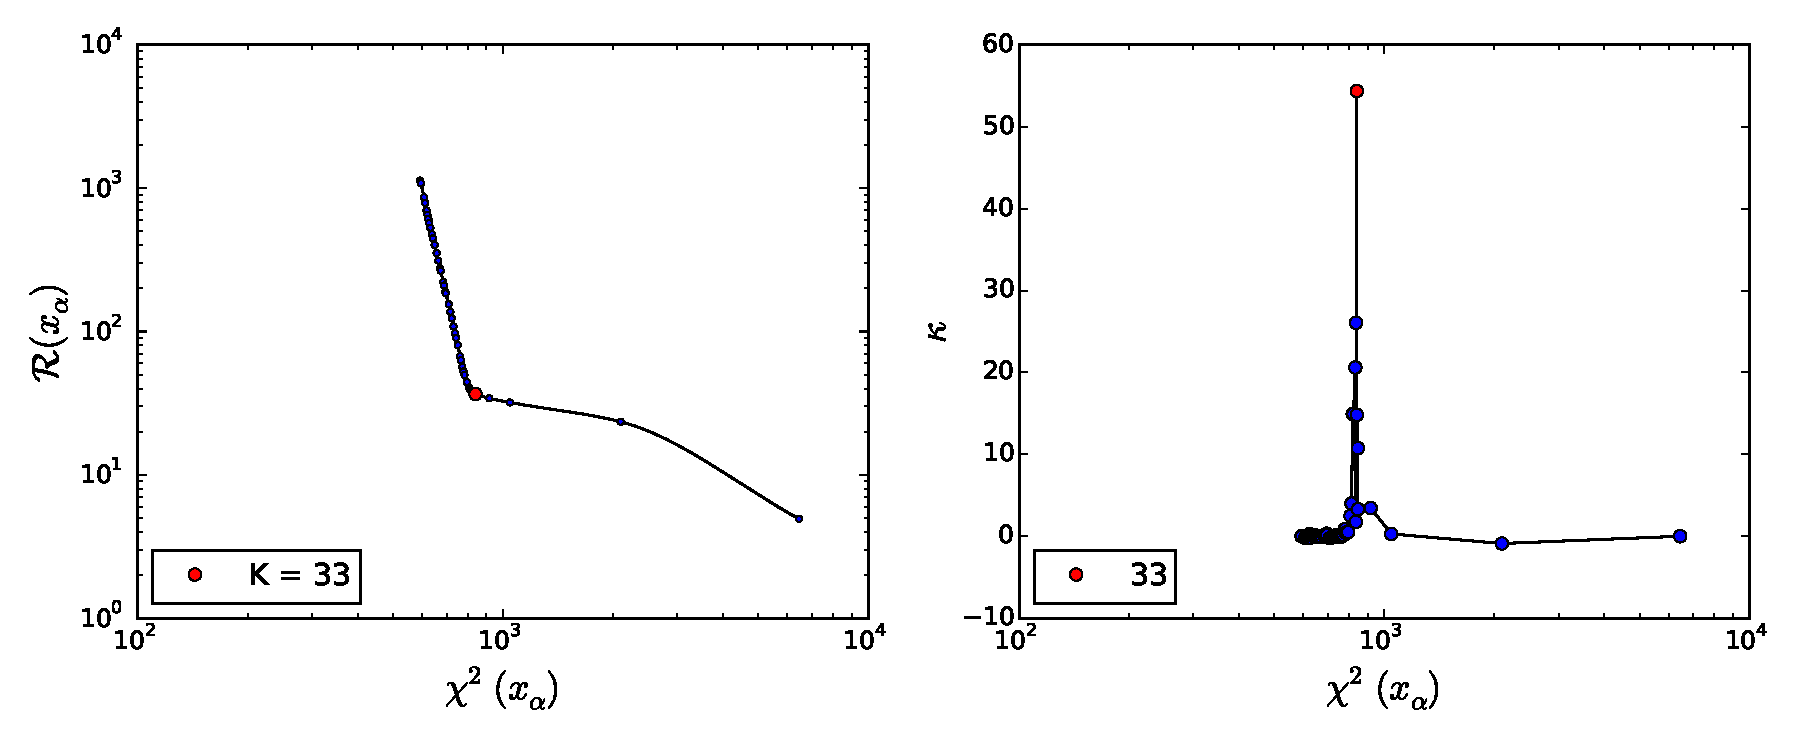
\includegraphics[width=0.95\textwidth]{inversion_methods/figure3.eps}
    \caption{Example of how to chose the hyper-parameter based on the L-curve method for the truncated SVD inversion method. The norm of the solution is used as a proxy for the regularizer. Left: loglog plot of the L-curve. Right: Curvature of the L-curve. The point of highest curvature/corner is indicated by the red point.}
    \label{fig:L_curve}
\end{figure}

\section{Benchmarks using Synthetic Data}\label{sec:results_synth}
In this section, we compare the different inversion methods using synthetic data calculated using Equation \ref{eq:wf_discrete} and known distribution functions. This enables us to compare the performance of the inversion methods using quantitative metrics since the true solutions are known.

\subsection{Benchmarking Apparatus}\label{sec:AUG_fida}
\subsubsection{Diagnostic Setup}
The benchmarking exclusively uses synthetic FIDA measurements. We base the diagnostic geometry on the FIDA systems installed at ASDEX Upgrade, which consists of five radial arrays each intersecting the Q3 neutral beam. From each system, a line of sight that views the center of the plasma is chosen (Fig. \ref{fig:FIDA_geometry}). 
\begin{figure}[ht]
    \centering
    \includegraphics[width=15cm]{inversion_methods/figure2.eps}
    \caption{Sketch of the geometry of the FIDA diagnostic set-up. a) Top view of the ASDEX Upgrade tokamak showing the NBI beam in grey and the FIDA lines-of-sight in colours. Only the lines-of-sight used here are shown. b) Poloidal cross-section showing that the FIDA measurement volume used here is slightly on the low-field side of the ASDEX Upgrade tokamak.} \label{fig:FIDA_geometry}
\end{figure}
The lines-of-sight originate from different positions in the plasma wall and intersect the neutral beam at approximately the same position---a requirement for Velocity-space Tomography.
Each view has a different angle between its line of sight and the magnetic field, probing different regions of the velocity space\cite{Salewski2014a}. In the plasma center, the respective angles are 14$^\circ$, 73$^\circ$, 103$^\circ$, 133$^\circ$ and 153$^\circ$.
Descriptions of ASDEX Upgrade's FIDA systems are found in Reference \cite{Weiland2015}.

\subsubsection{Test Distributions}
Three different velocity distributions are investigated: a Gaussian distribution, a bi-Maxwellian distribution, and a  NBI-distribution simulated by TRANSP/NUBEAM\cite{Pankin2004}. The three distributions are shown in Figure \ref{fig:original_distributions}. These three distribution functions pose different challenges to the inversion methods.
The Gaussian distribution represents a localized source of fast ions, a proxy for the peaks at the injection energies found in the distributions of neutral beam heated discharges. 
The bi-Maxwellian is a wide function covering the entire pitch range. Here the challenge is to recreate the large-scale structure. Lastly, we study a neutral beam injection distribution function. This is an important test case as it should be very similar to the distribution functions in experiments with NBI heating. The challenge here is the structural complexity on both small and large scales. 
\begin{figure}[h!]
    \centering
    \subfigure[Gaussian.\label{fig:orig_blob}]{%
    	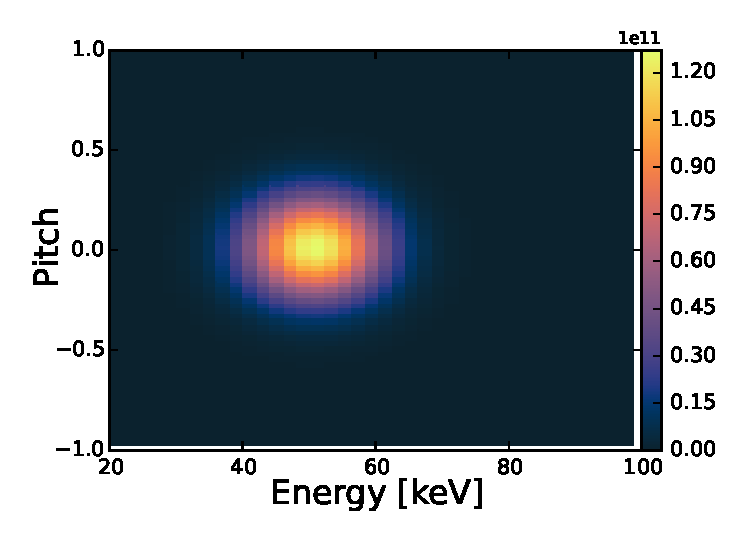
\includegraphics[width=0.30\textwidth]
    	{inversion_methods/figure4a.eps}
    }
    \subfigure[Bi-Maxwellian.\label{fig:orig_bimax}]{%
    	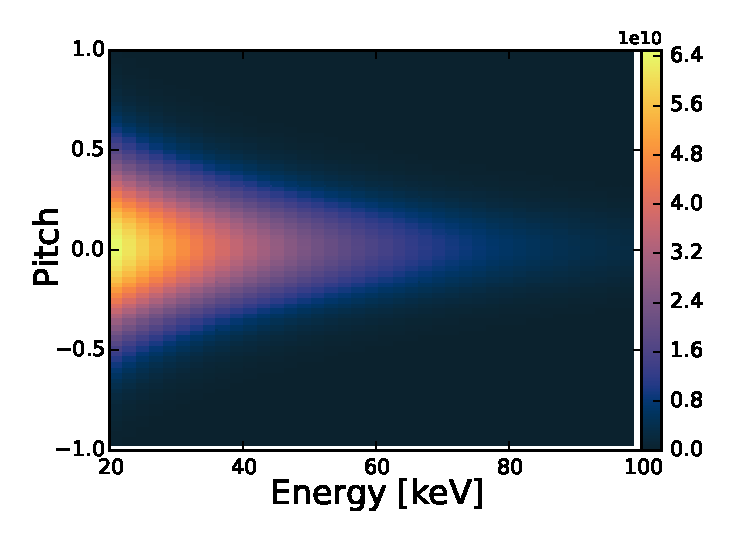
\includegraphics[width=0.30\textwidth] 
    	{inversion_methods/figure4b.eps}
    }
    \subfigure[NBI.\label{fig:orig_transp}]{%
    	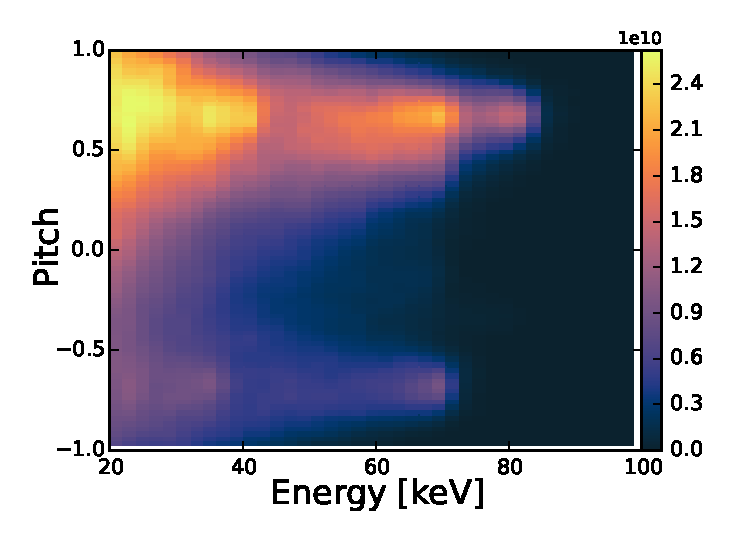
\includegraphics[width=0.30\textwidth] 
    	{inversion_methods/figure4c.eps}
    }
    \caption{Test velocity distributions functions as a function of energy and pitch. The functions are given in units of [ions/keV/cm$^3$]} \label{fig:original_distributions}
\end{figure}

\subsubsection{Simulating Measurement Noise}\label{sec:uncertainty}
A realistic model of spectra noise is used in the benchmarking. The photon noise of FIDA light scales approximately with the square root of the signal. However, in the absence of FIDA light the photon noise is dominated by the amount of bremsstrahlung, $B$; setting a lower limit on the noise level. 
These two effects are modeled as
\begin{equation}\label{eq:S_noisy}
    S_{\rm{noisy}} = S_{\rm{true}} + k \left\langle \sqrt{S_{\rm{true}}} \right\rangle \eta \quad \eta \sim \mathcal{N}(0,\max\left(\sqrt{B},\sqrt{S_{\rm{true}}}\right)) ,
\end{equation}
where $S_{\rm{noisy}}$ is the noisy spectrum, $S_{\rm{true}}$ is the true noise-free spectrum, $\left\langle \right\rangle$ denotes a mean, and $k$ is a scaling constant that allows us to vary the noise level.
By varying the noise level, we can investigate how robust the methods are against noise. Figure \ref{fig:spectra_transp} shows examples of the standard deviation of the synthetic spectra calculated using the NBI test distribution for $k=0.1$, $k=0.5$ and $k=0.9$. 
The noise level of actual FIDA measurements depends on the plasma parameters; a $k$ value in the range 0.3-0.5 represents the typical noise level in a discharge.
\begin{figure}[h!]
    \centering
    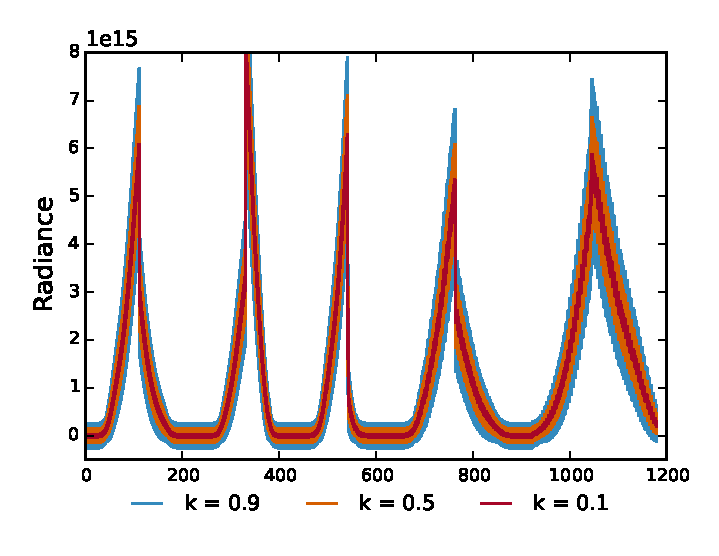
\includegraphics[width=0.70\textwidth]
    {inversion_methods/figure5.eps}
    \caption{Examples of the average noise levels in the synthetic spectra calculated using the NBI test distribution and equation (\ref{eq:S_noisy}) for k=\{0.1, 0.5 and 0.9\}. The width of the spectra corresponds to the standard deviation of the noise for the given $k$-value.}
    \label{fig:spectra_transp}
\end{figure}

\subsection{Quantitative Comparison Metrics}
The noise in the synthetic spectra propagates through the inversion process. If a single synthetic spectra is used, one of the inversion methods could get lucky and perform better then the rest.
In order to quantify the \textit{average} performance of the inversion methods, the results of the inversion methods are averaged over an ensemble of 25 noisy spectra. The variance of the reconstructions is used to quantify the effects of noise.

The inversion method itself also introduces a type of error. For instance, an inversion method may systematically bias solutions to be overly smooth. We can quantify this bias by finding the difference between the mean distribution for a given $k$ and the true distribution:
\begin{equation}\label{eq:bias}
    \mathrm{bias} = \mathbf{\hat{f}}_\mu - \mathbf{f}_{\rm{true}} \, , 
\end{equation}
where $\mathbf{\hat{f}}_\mu$ is the mean distribution and $\mathbf{f}_{\rm{true}}$ is the true distribution. 
Combining the bias with the variance, we define a measure of the total uncertainty of a pixel by the mean squared error, MSE, given by
\begin{equation}\label{eq:MSE}
    \mathrm{MSE} = \mathrm{variance} + \mathrm{bias}^2 \, .
\end{equation}

The MSE summed over the inversion along with the ratio of the inferred to the true fast-ion density are used as quantitative performance metrics.

\subsection{Inversion Results}
\subsubsection{Gaussian Distribution}
Figure \ref{fig:tomos_blob} shows reconstructions of the Gaussian distribution calculated with the different inversion methods for various noise levels. 
All methods reconstruct the position of the Gaussian distribution well. The characteristic widths of the Gaussians are approximately right but tend to be slightly larger than in the original test distribution. Measurement noise enhances this trend. We further observe the appearance of jitter in the reconstructions throughout velocity space. 
The minimum Fisher information and maximum entropy regularization methods stand out from the other methods in that they resemble the original function the most and exhibit the least jitter. This suggests superior resolution performance of these methods. Table \ref{tab:synthetic_parameters_blob} contains the true center coordinates and width of the Gaussian distribution in both energy and pitch. Furthermore, it contains the values obtained from the $k=0.5$ reconstructions calculated using the five different methods. All methods find the center coordinates well. The minimum Fisher information and maximum entropy methods produce significantly more peaked distributions, which is seen in their ability to better match the true width of the Gaussian. 
\begin{table}[h!]
    \caption{\label{tab:synthetic_parameters_blob} Parameters of the Gaussian test distribution. Parameters are found by fitting the reconstructed distributions to the analytic form of the true distribution.}
    \resizebox{\textwidth}{!}{\begin{tabular}{@{}r|llllll}
     & \textbf{True} & \textbf{SVD} & \textbf{T0} & \textbf{T1} & \textbf{MFI} & \textbf{ME} \\
    \hline\hline
    $\mu_E$ [keV] & 50 & 49.37$\pm$0.22 & 49.55$\pm$0.19 & 48.57$\pm$0.21 &  48.45$\pm$0.06 & 50.78$\pm$0.07 \\
    $\sigma_E$ [keV] & 10 & 15.16$\pm$0.32 & 15.34$\pm$0.27 & 16.61$\pm$0.30 & 11.24$\pm$0.08 & 8.87$\pm$0.10 \\
    $\mu_p$ [-] & 0 & 0.008$\pm$0.005 & -0.001$\pm$0.004 & -0.001$\pm$0.004 & -0.011$\pm$0.001 & 0.035$\pm$0.002 \\
    $\sigma_p$ [-] & 0.25 & 0.325$\pm$0.007 & 0.329$\pm$0.006 & 0.317$\pm$0.006 & 0.228$\pm$0.02 & 0.242$\pm$0.003 \\
    \hline
    \end{tabular}}
\end{table}

\begin{figure}[h!]
    \centering
    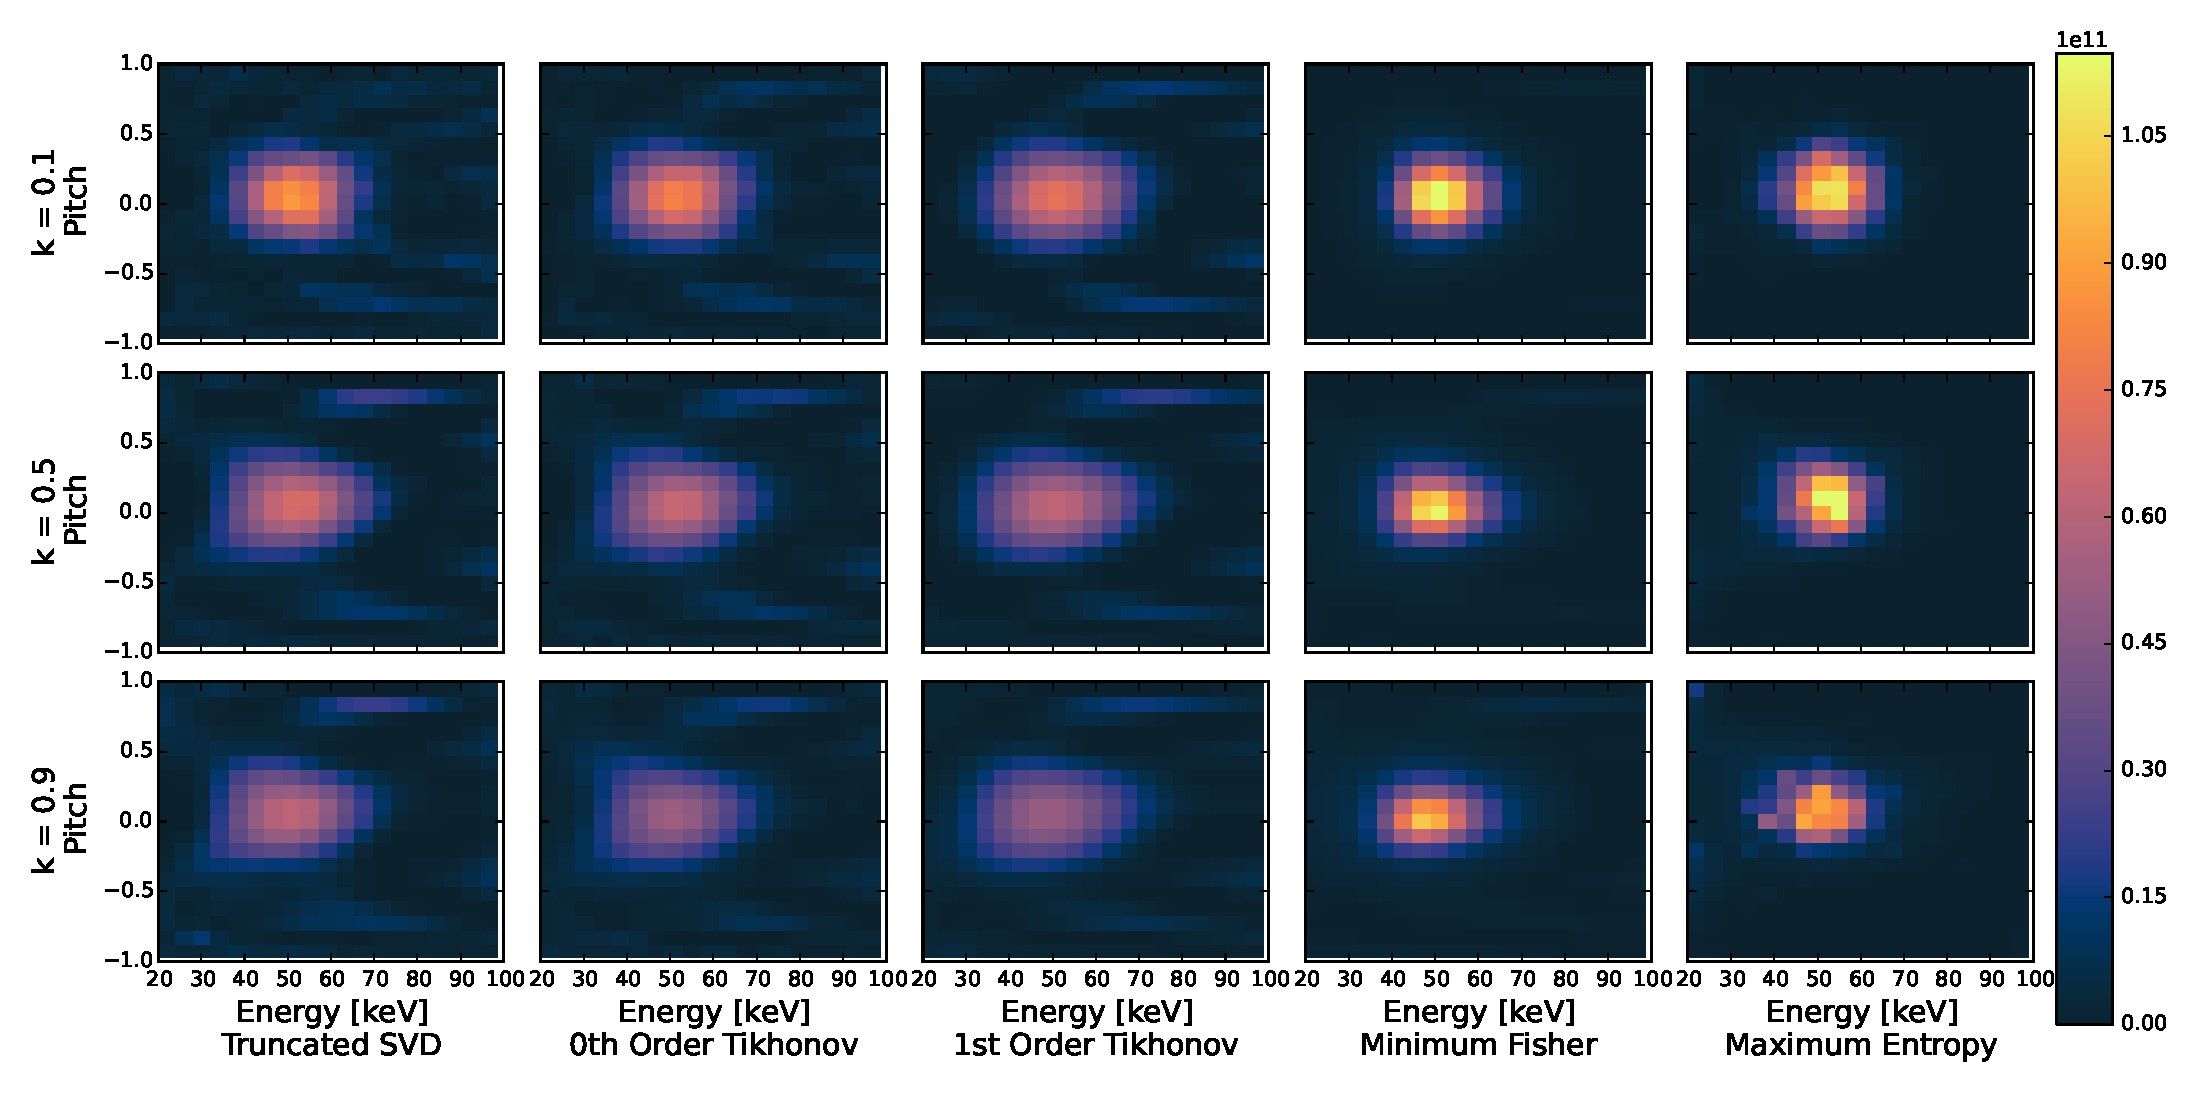
\includegraphics[width=0.95\textwidth]{inversion_methods/figure6.eps}
    \caption{Reconstructions of the Gaussian distribution (Fig. \ref{fig:orig_blob}) from on synthetic measurements using various inversion methods and noise levels. The noise level $k$ is defined in equation (\ref{eq:S_noisy}). Distributions have units of [ions/keV/cm$^3$] } 
    \label{fig:tomos_blob}
\end{figure}

\subsubsection{Bi-Maxwellian Distribution}
Figure \ref{fig:tomos_bimax} shows the reconstructions of the bi-Maxwellian distribution function. The large-scale shape of the distribution is reproduced by all five inversion methods. The pitch angle symmetry and long tail at $p=0$ is also reproduced.
The first-order Tikhonov, minimum Fisher information, and maximum entropy methods reproduce the distribution particularly well. Table \ref{tab:synthetic_parameters_bimax} contains the true parallel and perpendicular temperatures used in calculating the bi-Maxwellian and the values obtained from fitting the $k=0.5$ reconstructions to the analytic form of the bi-Maxwellian. For the bi-Maxwellian distribution, the minimum Fisher information method most closely recreates the true values.
\begin{table}[h!]
    \caption{\label{tab:synthetic_parameters_bimax} Parameters of the bi-Maxwellian test distribution. Parameters are found by fitting the reconstructed distributions to the analytic form of the true distribution.}
    \resizebox{\textwidth}{!}{\begin{tabular}{@{}r|llllll}
     & \textbf{True} & \textbf{SVD} & \textbf{T0} & \textbf{T1} & \textbf{MFI} & \textbf{ME} \\
    \hline\hline
    $E_\parallel$ [keV] & 3 & 5.12$\pm$0.19 & 5.34$\pm$0.18 & 4.98$\pm$0.09 & 2.94$\pm$0.06 & 4.09$\pm$0.13 \\
    $E_\perp$ [keV] & 20 & 24.36$\pm$0.73 & 26.26$\pm$0.73 & 23.79$\pm$0.35 & 22.51$\pm$0.32 & 24.73$\pm$0.61 \\
    \hline
    \end{tabular}}
\end{table}
\begin{figure}[h!]
    \centering
    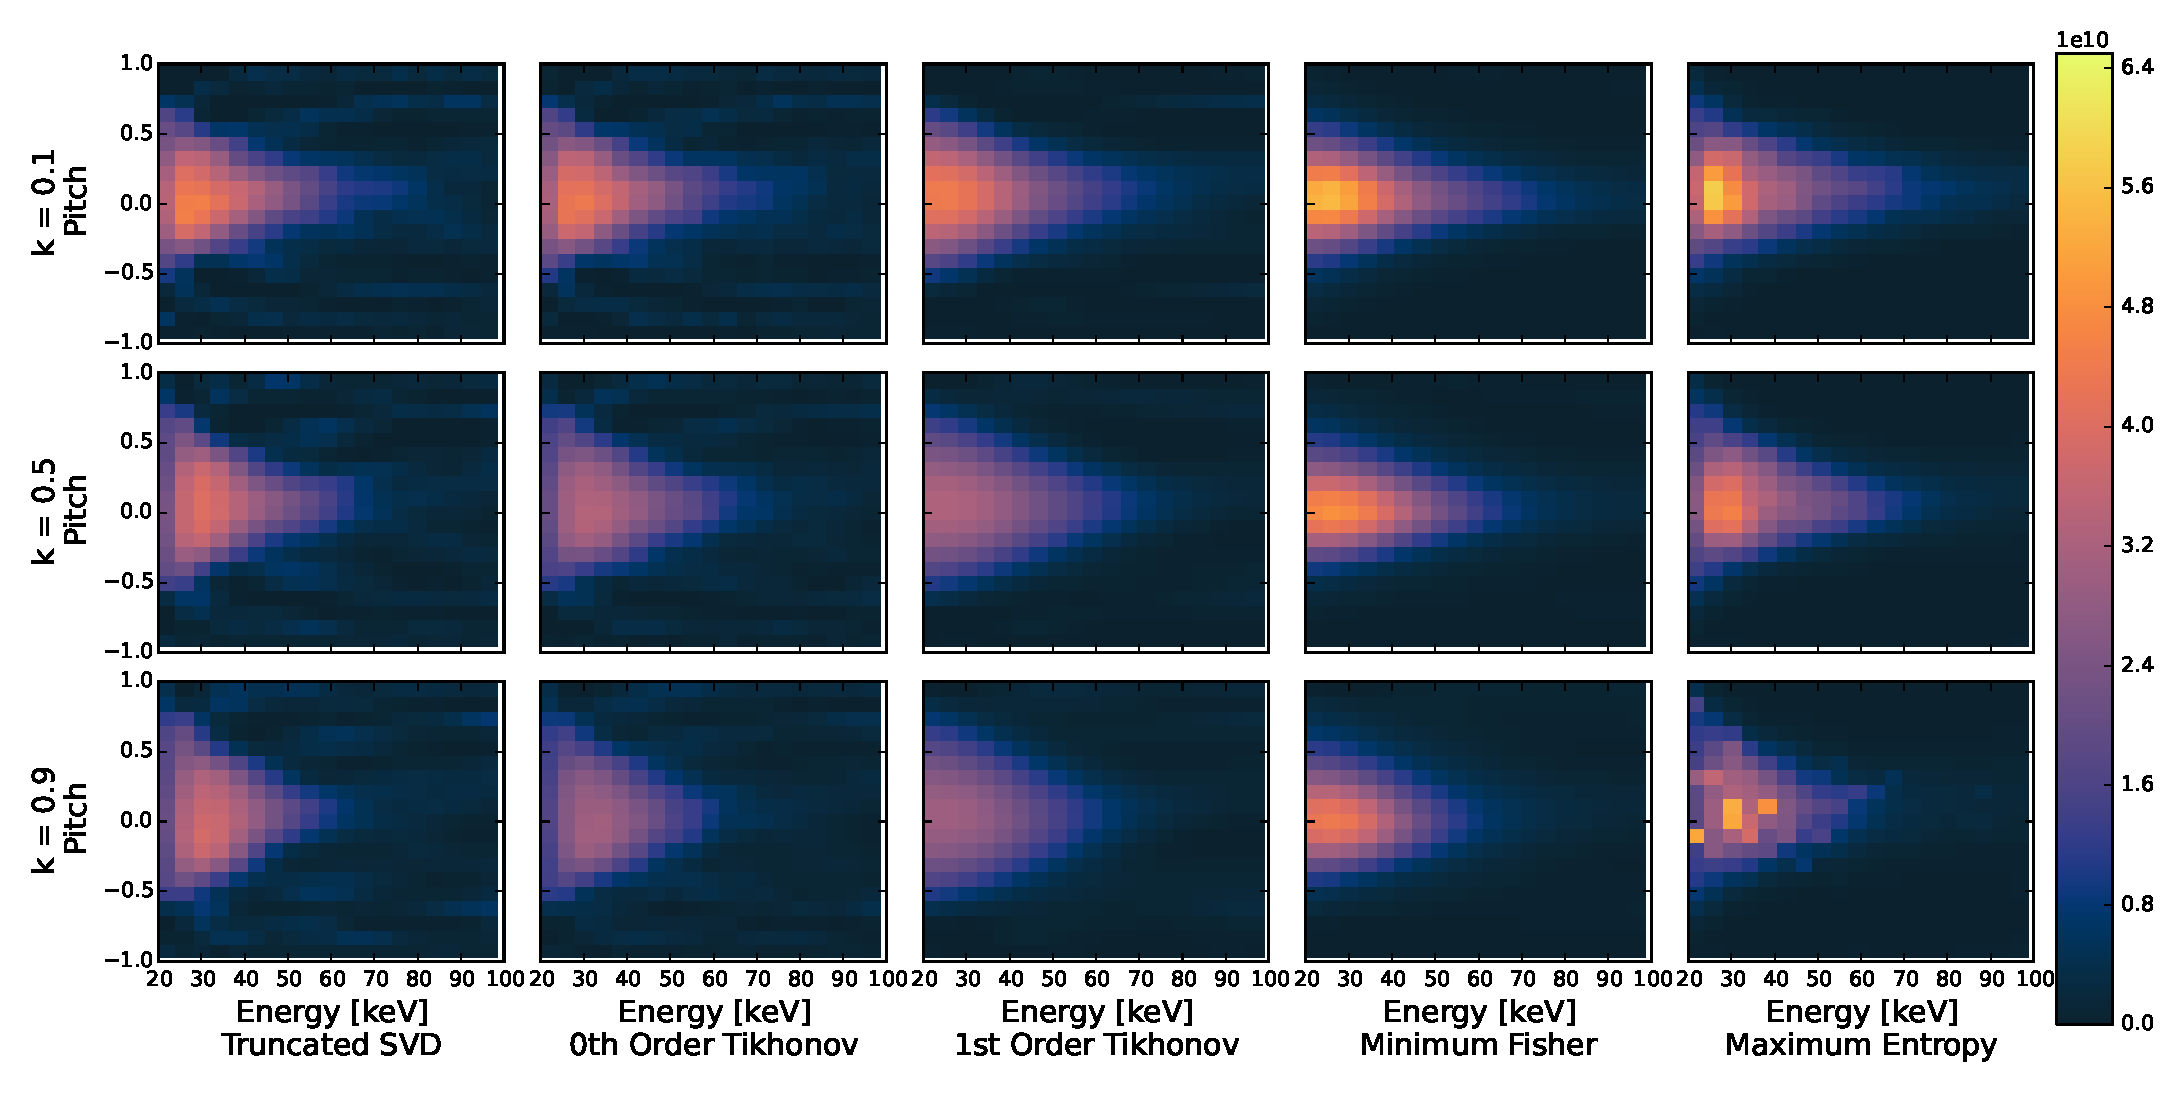
\includegraphics[width=0.95\textwidth]{inversion_methods/figure7.eps}
    \caption{Reconstructions of the bi-Maxwellian (Fig. \ref{fig:orig_bimax}) distribution from synthetic measurements using various inversion methods and noise levels. The noise level $k$ is defined in equation (\ref{eq:S_noisy}). Distributions have units of [ions/keV/cm$^3$] }
    \label{fig:tomos_bimax}
\end{figure}

\subsubsection{NBI Distribution}
Figure \ref{fig:tomos_transp} shows reconstructions of the NBI distribution function for various noise levels and inversion methods.
This fast-ion distribution function is typical for neutral beam injection with two co-current beams with injection energies at 80 keV and 70 keV and one counter-current beam with an injection energy of 70 keV. 
Therefore, this distribution function is a more difficult test case. 
The overall shape of the NBI distribution function is reproduced by all five inversion methods. The protrusion at pitches of about 0.7 originates from the co-current beam injection, and the weaker protrusion at pitches of -0.7 originate from the counter-current beam injection. All reconstructions show the full energy beam injection peak for co-current injection (positive pitch) at larger energies than that for counter-current injection (negative pitch). 
The first-order Tikhonov, minimum Fisher information and maximum entropy regularization results in smooth reconstructions. This makes the overall shape of the function with protrusions at positive and negative pitches stand out most clearly. 
The local maxima due to the beam injection peaks at full, half and third energies are recreated by the maximum entropy method in the case of low noise ($k=0.1$). They are also visible in the SVD and zeroth-order Tikhonov tomographies at low noise; however, the peaks are accompanied by other artifacts.
For larger noise levels, none of the methods are able to resolve more than one peak.
\begin{figure}[h!]
    \centering
    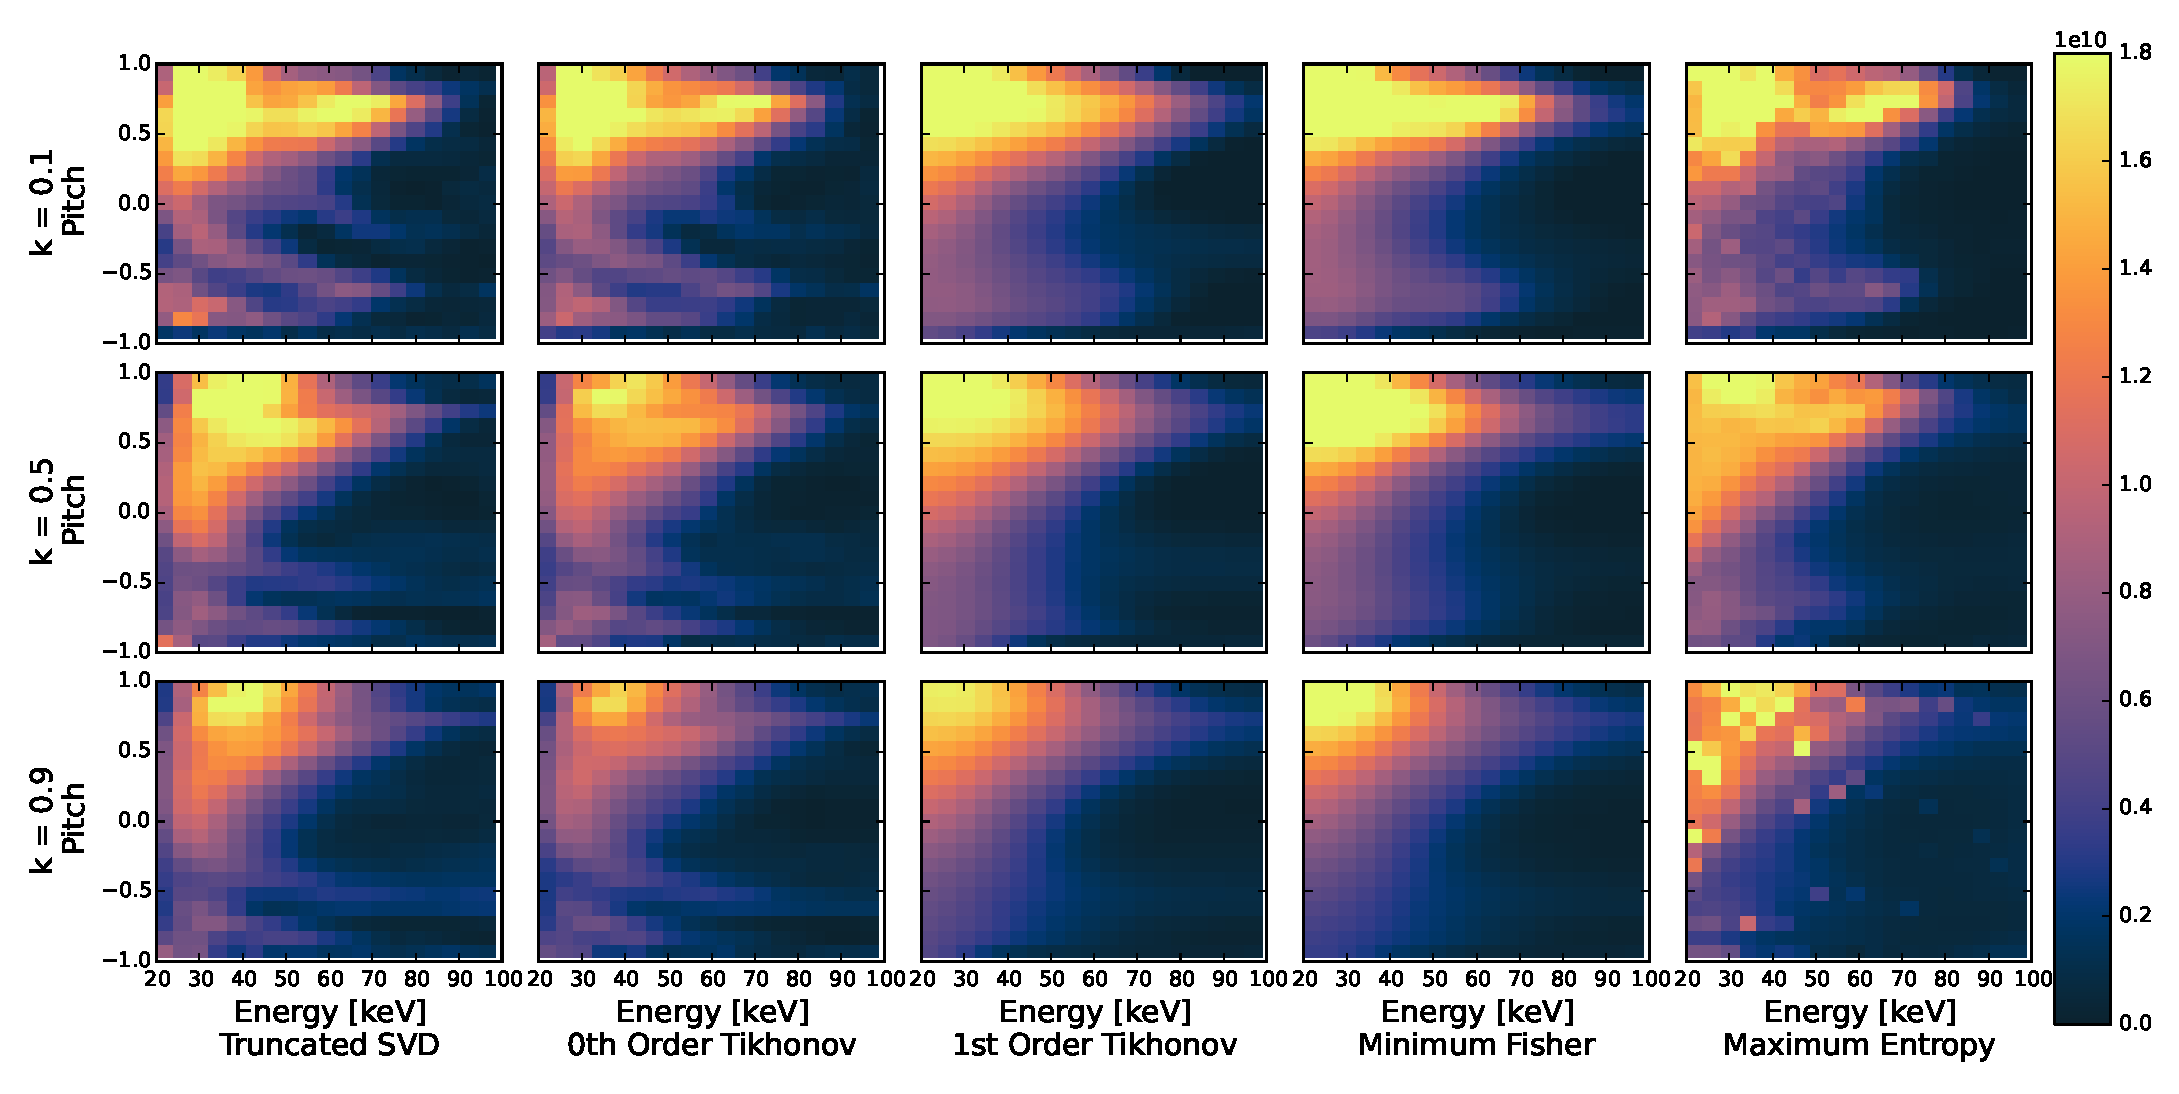
\includegraphics[width=0.95\textwidth]{inversion_methods/figure8.eps}
    \caption{Tomographies of the beam distribution from figure \ref{fig:orig_transp} in units of [ions/keV/cm$^3$] based on synthetic measurements using various inversion methods and noise levels. The noise level $k$ is defined in equation (\ref{eq:S_noisy}).} \label{fig:tomos_transp}
\end{figure}

The uncertainties of the reconstructions of the NBI distribution are shown in Figure \ref{fig:uncertainties_transp} for a noise level of $k=0.5$.
The top row shows the square root of the variance of the reconstructions. 
Compared with the values of the reconstructions in Figure \ref{fig:tomos_transp}, the uncertainties are about one order of magnitude smaller; the smallest for first-order Tikhonov and minimum Fisher information regularization. 
The middle row shows the bias.
Negative values denote regions where too few ions are placed, positive values denote regions where too many ions are placed.
The beam peaks are seen in the bias, especially for first-order Tikhonov, minimum Fisher information and maximum entropy regularization as these are only able to resolve the peaks for low noise levels.
The last row shows the square root of the mean squared error. 
The main contribution to the uncertainty is the bias.
\begin{figure}[h!]
    \centering
    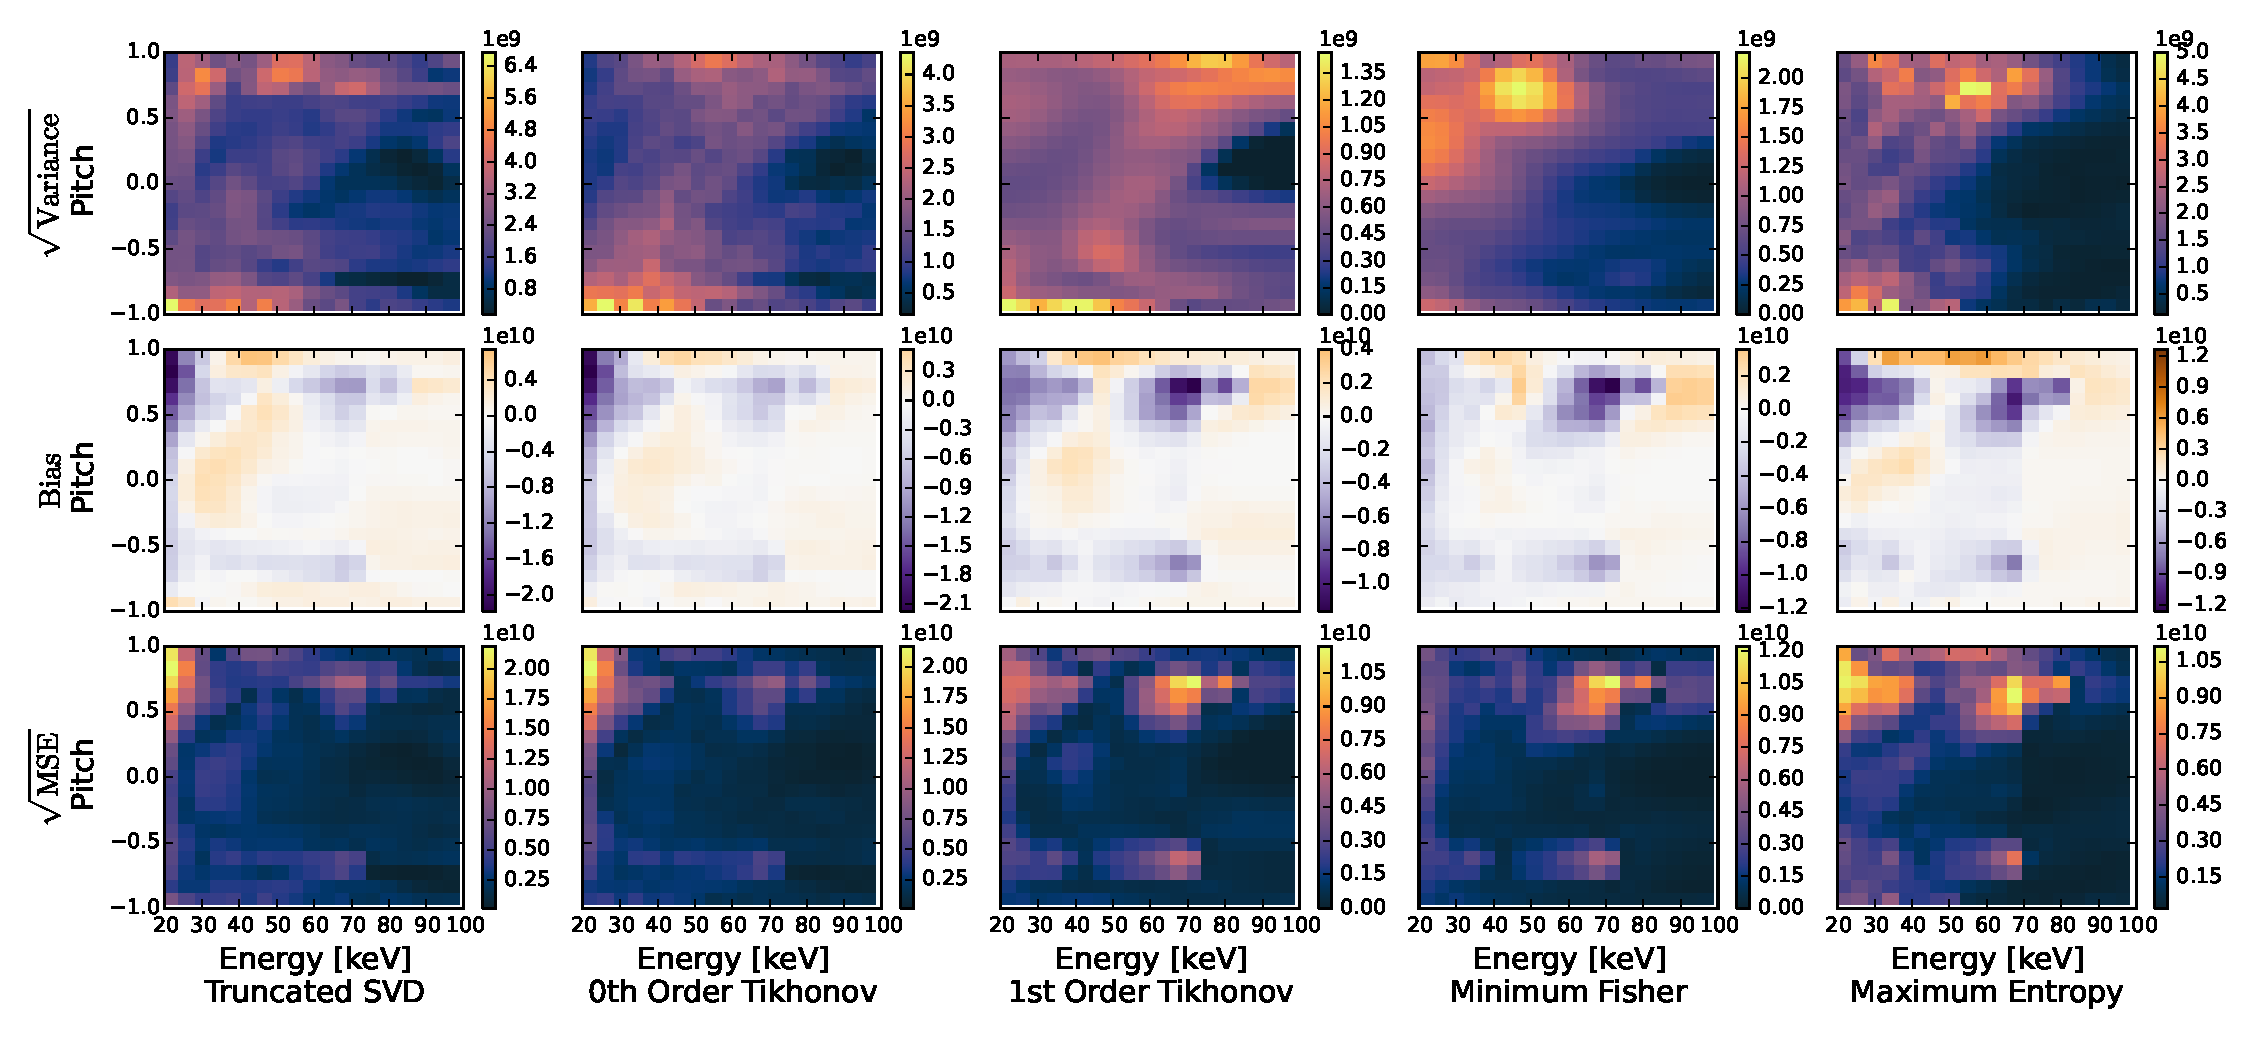
\includegraphics[width=0.95\textwidth]{inversion_methods/figure10.eps}
    \caption{Uncertainties for the reconstructions of the beam distribution in units of [ions/keV/cm$^3$]. All uncertainties are calculated for a noise level of $k=0.5$.}
    \label{fig:uncertainties_transp}
\end{figure}

\subsubsection{Noise Scaling}
Figure \ref{fig:Qfigs_tomos} shows the behaviour of the performance parameters as a function of noise level. Figures \ref{fig:Q1_blob}, \ref{fig:Q1_bimax} and \ref{fig:Q1_transp} show the total mean squared error.
The mean squared error increases for larger noise levels for all inversion methods and test distributions. 
The minimum Fisher information regularization method has the lowest mean squared error for all test distributions. 
Figures \ref{fig:Q2_blob}, \ref{fig:Q2_bimax} and \ref{fig:Q2_transp} show the density ratios. The general trend is that the methods produce a lower density ratio for large error levels. Thus, for very large noise levels the absolute values of an inferred density obtained from a reconstruction might be unreliable. For the Gaussian test distribution, the minimum Fisher information and maximum entropy methods are very good at recreating the correct density. The other three methods overestimate the amount of ions present. This is also the case for the bi-Maxwellian distribution but not to the same extent. 
For the NBI test distribution, the spread in densities is smaller than for the other cases.
\begin{figure}
    \centering
    \subfigure[Total MSE, Gaussian\label{fig:Q1_blob}]{%
    	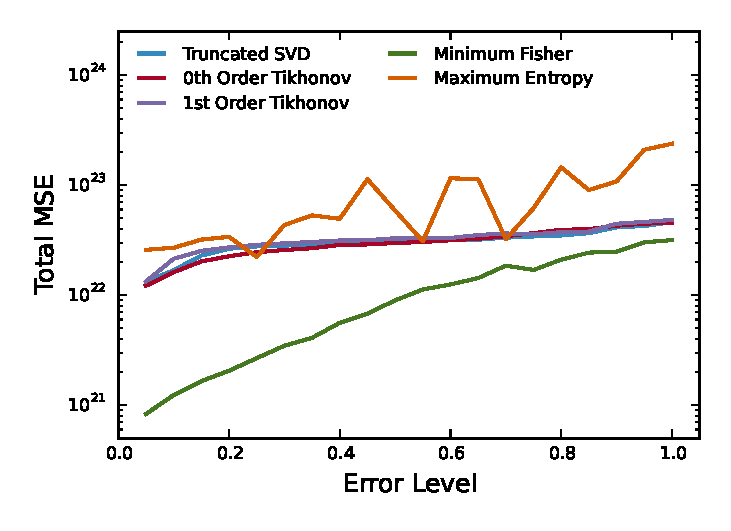
\includegraphics[width=0.45\textwidth]{inversion_methods/figure9a.eps}	
    }
    \subfigure[Density ratio, Gaussian\label{fig:Q2_blob}]{%
    	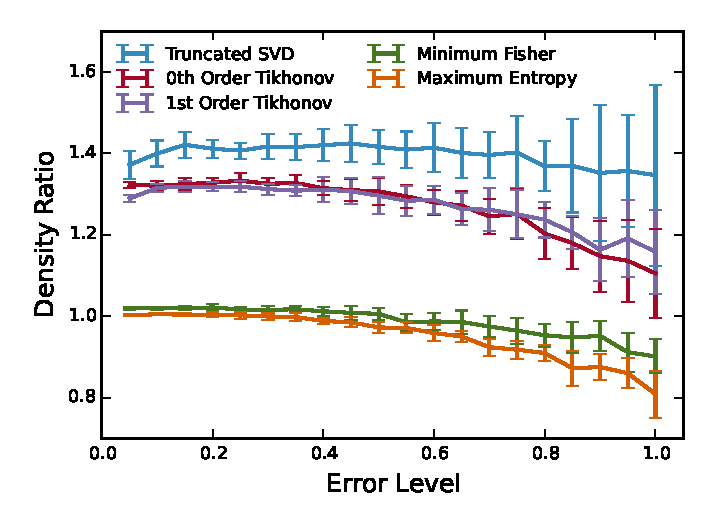
\includegraphics[width=0.45\textwidth]{inversion_methods/figure9b.eps}
    }
    \subfigure[Total MSE, bi-Maxwellian\label{fig:Q1_bimax}]{%
    	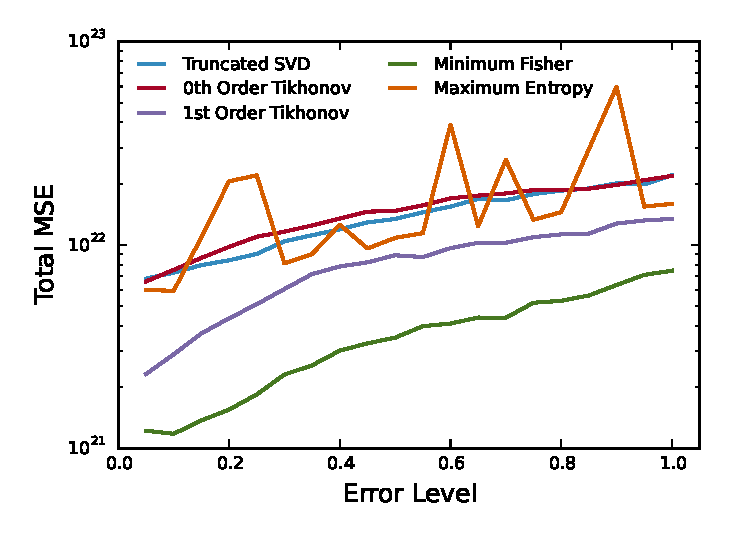
\includegraphics[width=0.45\textwidth]{inversion_methods/figure9c.eps}
    }
    \subfigure[Density ratio, bi-Maxwellian\label{fig:Q2_bimax}]{%
    	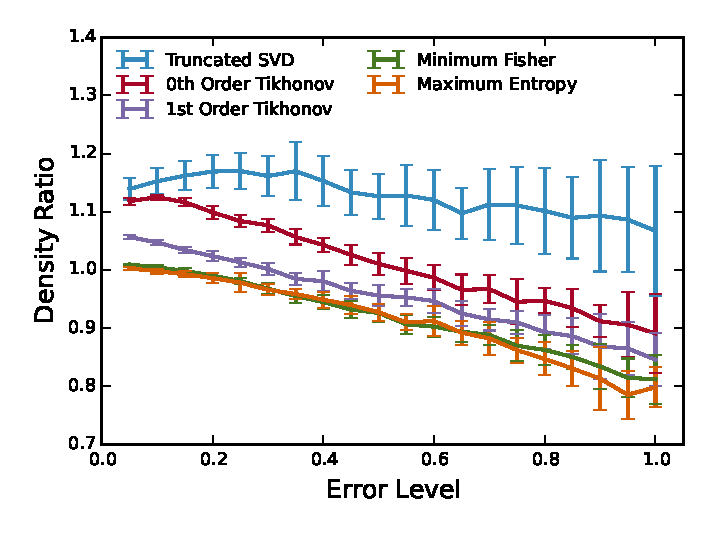
\includegraphics[width=0.45\textwidth]{inversion_methods/figure9d.eps}
    }
    \subfigure[Total MSE, NBI\label{fig:Q1_transp}]{%
    	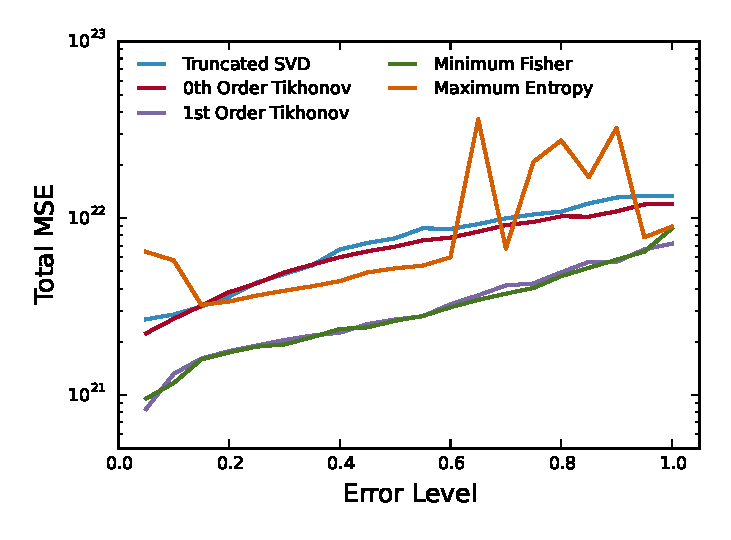
\includegraphics[width=0.45\textwidth]{inversion_methods/figure9e.eps}
    }
    \subfigure[Density ratio, NBI\label{fig:Q2_transp}]{%
    	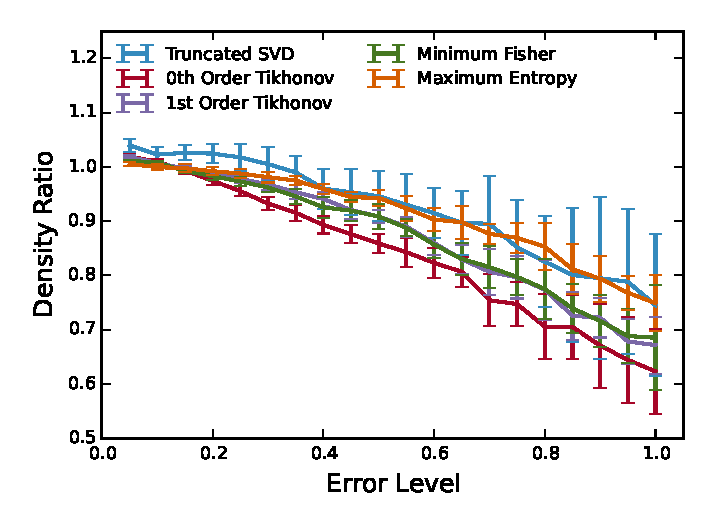
\includegraphics[width=0.45\textwidth]{inversion_methods/figure9f.eps}
    }
    \caption{Noise scaling of the reconstructions of the test distributions. The left column shows the total mean squared error. The right column shows the density ratio. }
    \label{fig:Qfigs_tomos}
\end{figure}

\section{Redistribution of Fast-ions by a Sawtooth Crash}\label{sec:results_real}
A sawtooth crash is a periodic plasma instability which can occur when the central safety factor drops below one. It changes the magnetic field topology and has been observed to redistribute particles and energy from the center of the plasma. Furthermore, it has been observed on several machines that passing fast ions are redistributed more strongly compared to trapped ions \cite{Nielsen2011,Muscatello2012,Geiger2015,weiland2016}.
Here we use the five different inversion methods to investigate the effect of a sawtooth on the central fast-ion population in ASDEX Upgrade. Figure \ref{fig:31557_timetraces} shows time traces from AUG discharge \#31557. The sawtooth crashes are evident in the central electron density as well as the central electron and ion temperatures. 
\begin{figure}[h!]
    \centering
    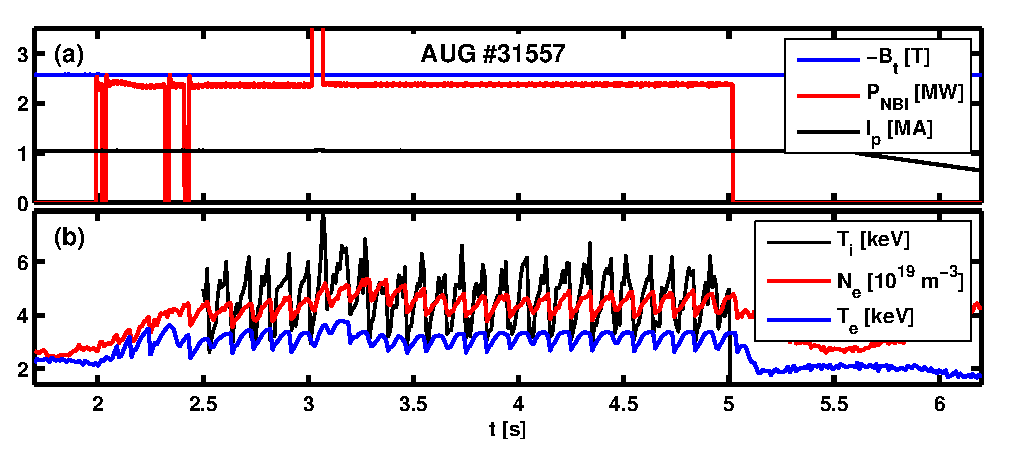
\includegraphics[width=0.75\textwidth]{inversion_methods/figure12.eps}
    \caption{Time traces of AUG discharge \#31557. a) Toroidal magnetic field, total injected NBI power and the plasma current. b) Ion and electron temperatures and electron density at $\rho_p=0.1$.} \label{fig:31557_timetraces}
\end{figure}
Experimental FIDA spectra from just before and after the sawtooth crash in ASDEX Upgrade discharge \#31557 at 2.25~s was used in this analysis. The same diagnostic setup used in the benchmarks is used here.
Figure \ref{fig:tomos_sawtooth} shows the reconstructed distributions from just before and after the crash. Figure \ref{fig:uncertainties_sawtooth} shows the uncertainties of the reconstructions of the pre-crash distribution.
\begin{figure}[h!]
    \centering
    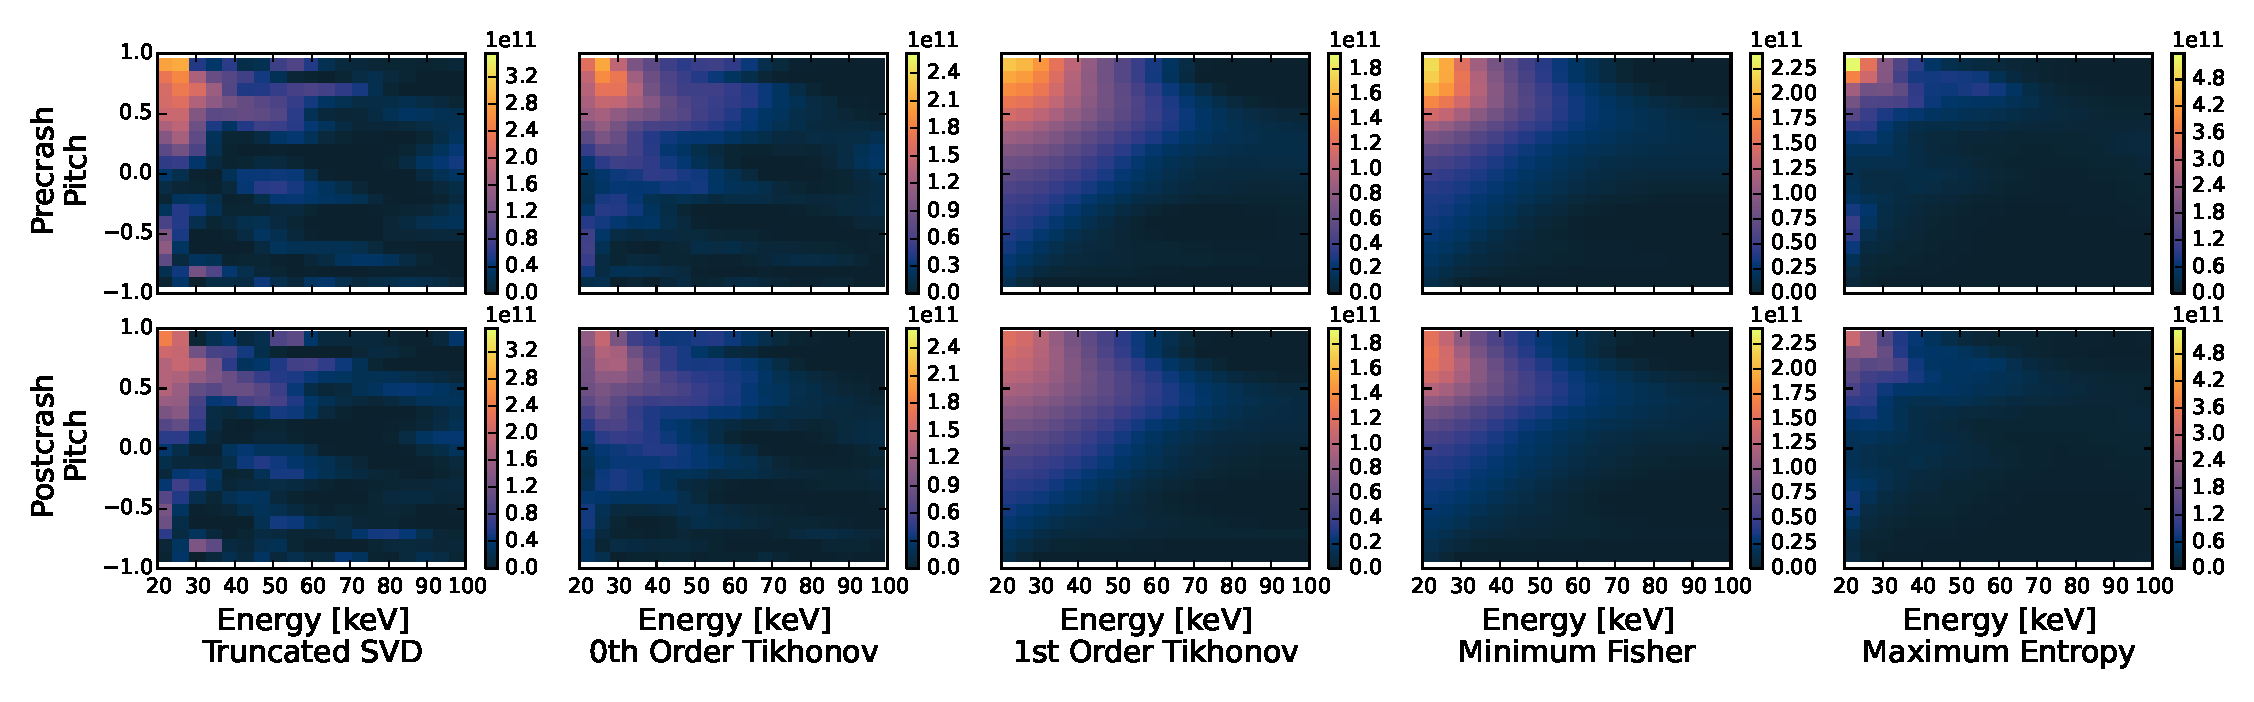
\includegraphics[width=0.95\textwidth]
    {inversion_methods/figure13.eps}
    \caption{Reconstructed fast-ion distributions before and after a sawtooth crash calculated using the different inversion methods.} \label{fig:tomos_sawtooth}
\end{figure}
\begin{figure}[h!]
    \centering
    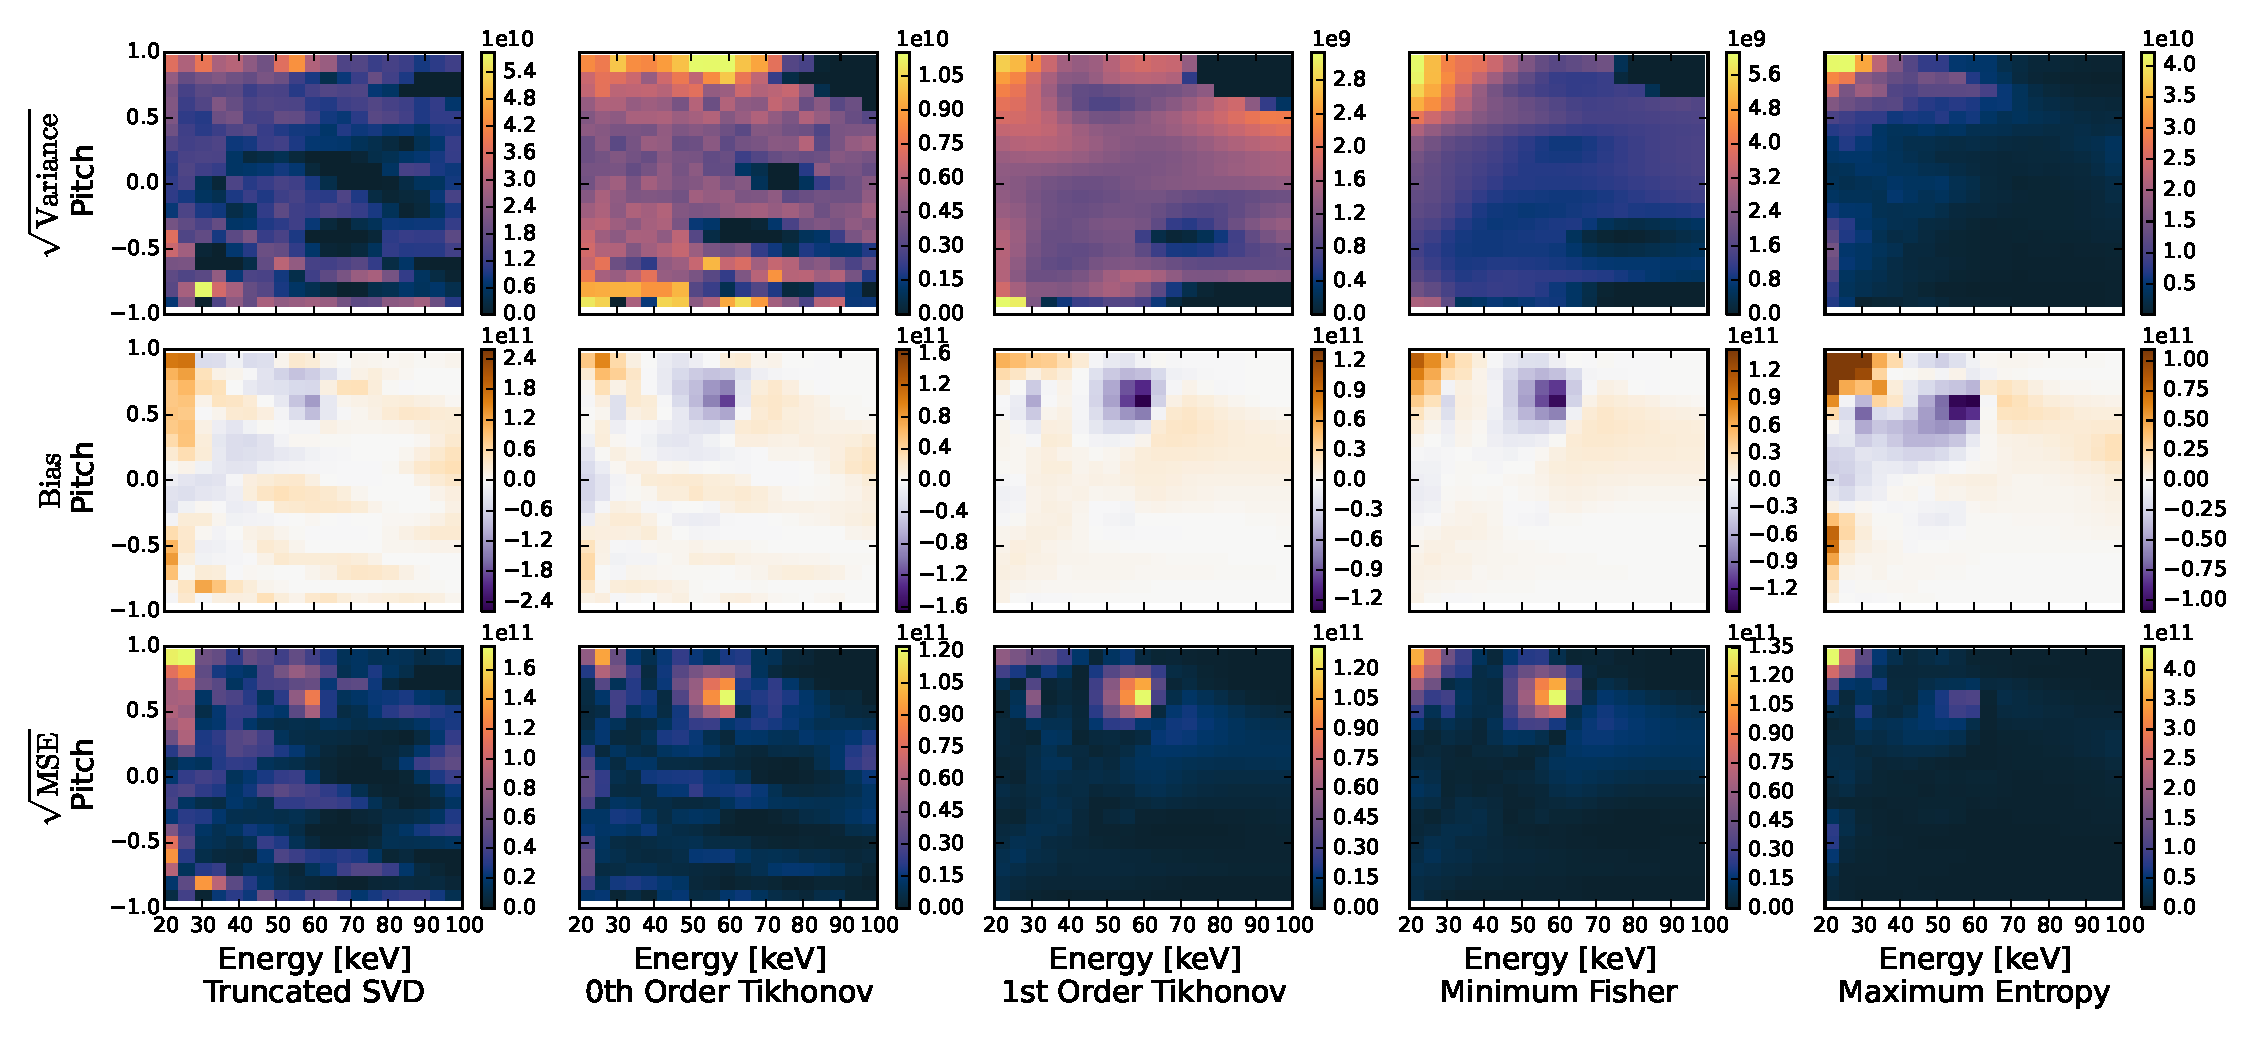
\includegraphics[width=0.95\textwidth]{inversion_methods/figure14.eps}
    \caption{Measures of uncertainties using the different regularization methods. The bias is calculated using the ``true'' distribution that is calculated using TRANSP's Kadomstev model.} \label{fig:uncertainties_sawtooth}
\end{figure}

The significant drop in fast ion density during the sawtooth crash is seen by all the inversion methods. By comparing the absolute values of the reconstructions with the uncertainties, we can identify the velocity-space regions where we can be confident in the result. 
Figure \ref{fig:tomos_sawtooth_normalized_with_MSE} shows the reconstructions normalized by $\sqrt{\mathrm{MSE}}$ for the five inversion methods. To calculate the bias after the sawtooth crash, the Kadomtsev model as implemented in TRANSP is used to model the effect of the sawtooth crash on the fast ions.
The parts of velocity space where the values are large correspond to regions where we are confident in the results and regions with low values correspond to uncertain regions. It is seen that the part of velocity space at the full energy peak at 60 keV is very uncertain for all inversion methods. This is because the methods are not able to resolve the peak given the choice of hyper-parameter. 
\begin{figure}[h!]
    \centering
    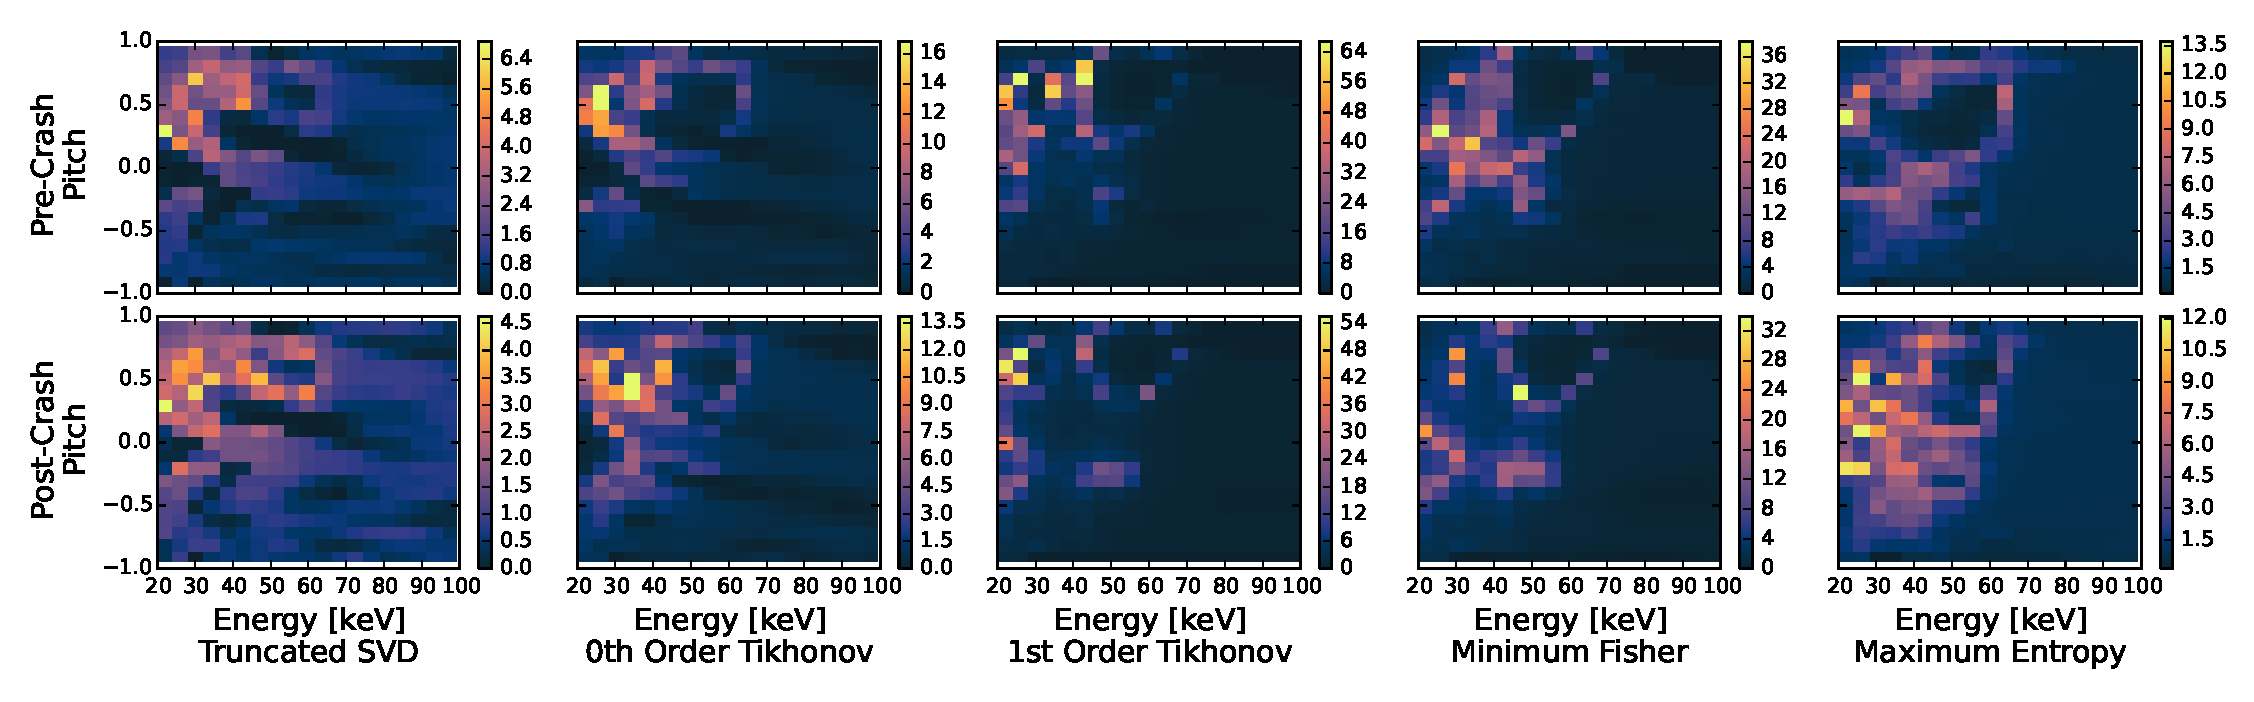
\includegraphics[width=0.95\textwidth]{inversion_methods/figure15.eps}
    \caption{Reconstructions of the ion velocity distribution normalized with $\sqrt{\mathrm{MSE}}$ before (top row) and after (bottom row) the sawtooth crash.}
    \label{fig:tomos_sawtooth_normalized_with_MSE}
\end{figure}
 
To further investigate the velocity-space dependence of the change in the fast-ion distribution function, we calculate the relative change:
\begin{equation}
\Delta \mathbf{\hat{f}}_{rel} = \frac{\mathbf{\hat{f}}_{after} - \mathbf{\hat{f}}_{before}}{\mathbf{\hat{f}}_{before}}  \, .
\end{equation}
The relative change is calculated for every regularization method and plotted in Figure \ref{fig:tomos_sawtooth_rel}. 
The top row shows the relative change as a function of energy and pitch. The bottom row shows the uncertainties of the relative change.
The variance of the relative change is calculated from an ensemble of relative changes, which was generated by sampling within the error bars of the experimental spectra.
\begin{figure}[h!]
    \centering
    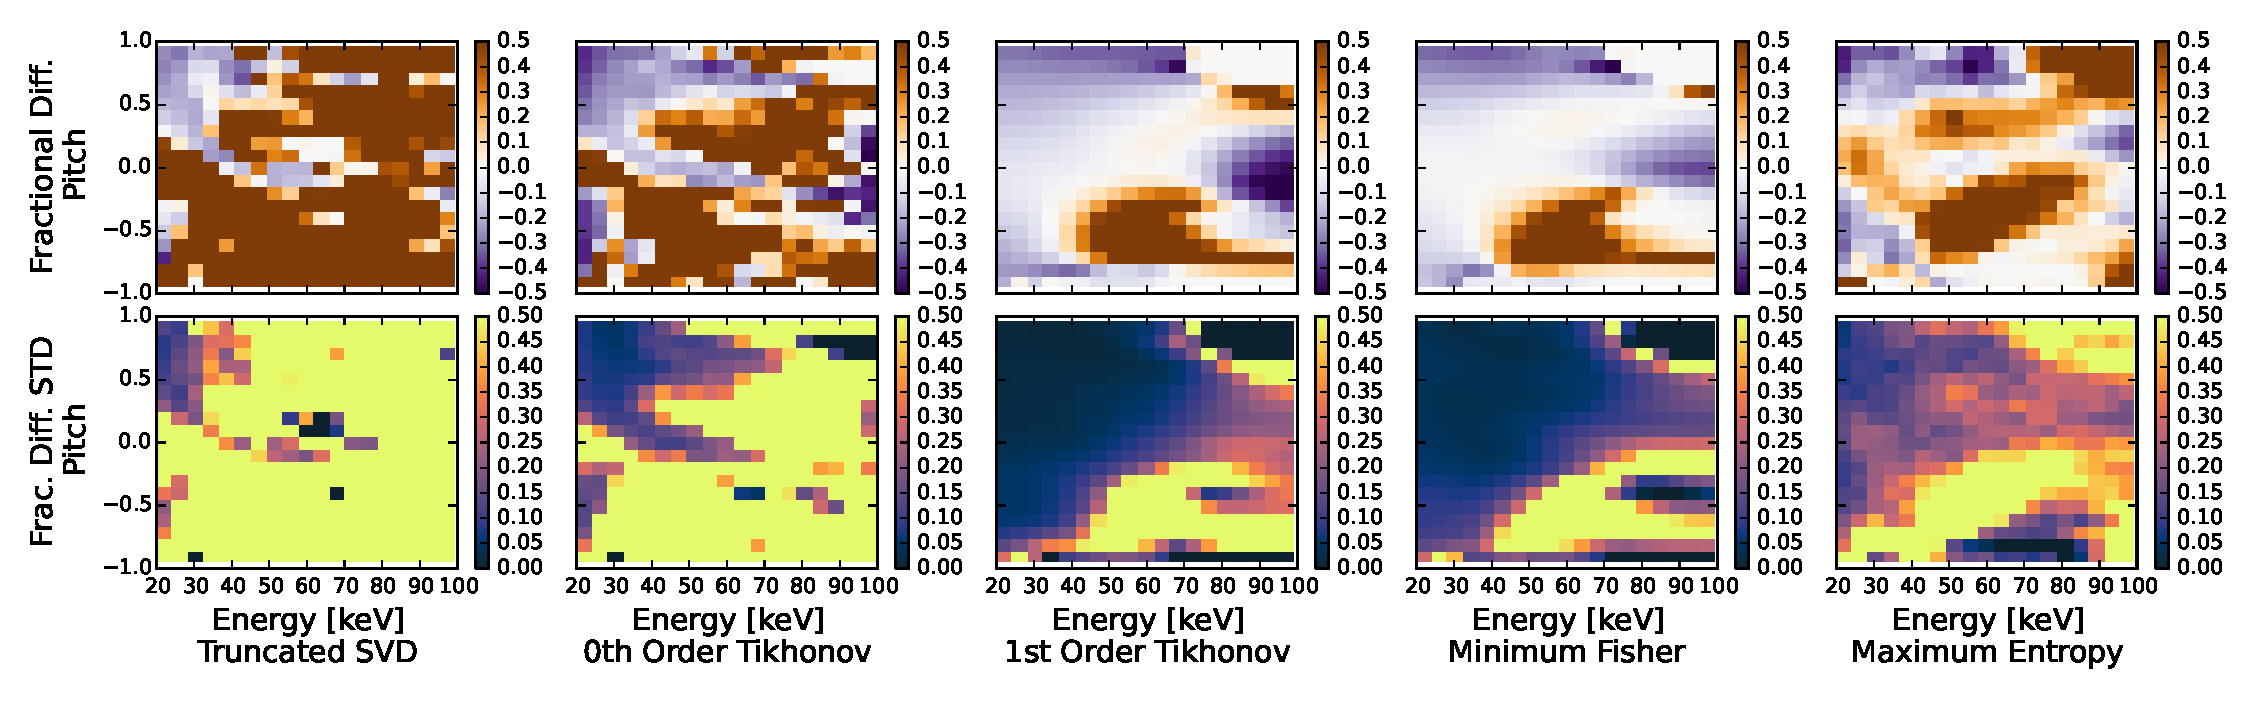
\includegraphics[width=0.95\textwidth]{inversion_methods/figure16.eps}
    \caption{Relative change of the fast-ion velocity distribution function.} \label{fig:tomos_sawtooth_rel}
\end{figure}
The velocity-space dependence of the relative change is especially clear in the first-order Tikhonov and the minimum Fisher information figures as the amount of jitter in these reconstructions is significantly smaller compared to the other methods. 
Both first-order Tikhonov and minimum Fisher information suggest that ions with large pitch values are redistributed more compared to ions with pitch close to zero. 
This trend is also confirmed by the singular value decomposition, zeroth-order Tikhonov and maximum entropy in the regions where the reconstructions are reliable.
The unreliable regions are shown as those with large standard deviation compared with amplitudes of the reconstructions. 
Similar trends were observed previously using singular value decomposition \cite{Geiger2015} and a variant of a first-order Tikhonov \cite{Weiland2015}.
Figure \ref{fig:tomos_sawtooth_rel_1D} shows the ratio of the post-crash distribution to the pre-crash distribution integrated over energy as a function of pitch for all five inversion methods. Thus, it is a measure of the pitch dependence of the change in the fast ion distribution function. 
For pitch values close to zero, all inversion methods except maximum entropy predict a redistribution level of between 10\% and 20\%.
For pitch values above 0.4, the redistribution level increases to between 30\% and 40\% as seen by all five inversion methods. For negative pitch values, where very few ions are present, it isn't possible to determine the amount of redistribution.
\begin{figure}[h!]
    \centering
    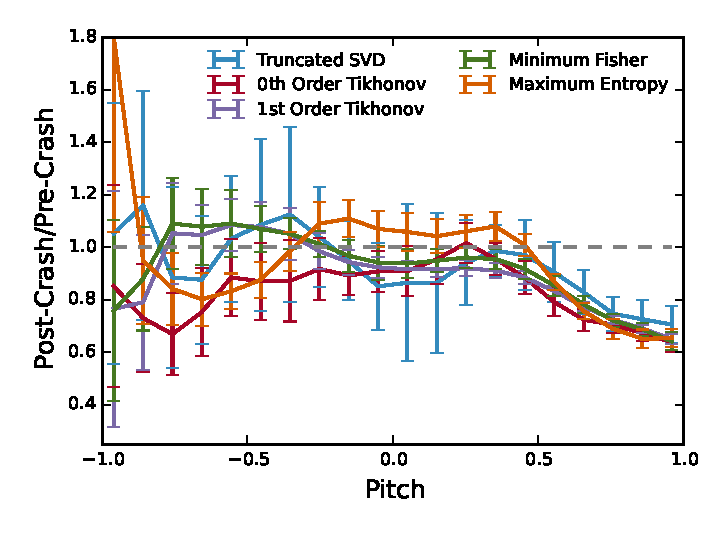
\includegraphics[width=0.70\textwidth]{inversion_methods/figure17.eps}
    \caption{Ratio of the fast-ion velocity-space distribution functions before and after the crash integrated over energy shown as a function of pitch.} \label{fig:tomos_sawtooth_rel_1D}
\end{figure}

\section{Discussion}
In order to calculate the true bias of a given reconstruction, it is necessary to know the true distribution. This makes it impossible to calculate the true bias of a reconstruction from experimental measurements. Here, we have used a TRANSP distribution and the Kadomtsev model to generate an estimate of the true distribution. 
However, in other cases it might not be possible to calculate a good quantitative estimate. 
In these cases, the best one can do is estimate a qualitative bias based on the general behavior of a inversion method.
On the other hand, uncertainties based solely on the propagation of measurement error through a given inversion method only represents the spread of obtainable solutions, and thus can be misleading since they can be made almost arbitrarily small, simply by over-regularizing.

When the noise level is not too large, 
the first-order Tikhonov, minimum Fisher information and maximum entropy regularization methods can reconstruct the overall shape of the true distribution function very well.
However, the first-order Tikhonov and minimum Fisher information methods lack capability to resolve very fine and detailed features.
For large noise levels, the maximum entropy has a tendency to produce solutions with large variances.
Truncated SVD and zeroth-order Tikhonov can resolve fine details, especially for measurements with low noise levels; however, they often produce features in wrong parts of velocity space.

It is seen that the absolute values of a derived quantity such as the fast-ion density depend on the noise level in the data. However, we find that the ratio of such quantities is less sensitive to the specific noise level and bias. Hence, we can make statements about changes in such quantities with greater confidence than about the absolute values themselves since biases introduced by the inversion methods will tend to cancel. For example, the bias in the reconstructions tends to be similar before and after a sawtooth crash, and hence it partly cancels in the relative change.
